\documentclass[a4paper,12pt]{article}
\usepackage{jheppub}
\renewcommand{\familydefault}{\rmdefault}
\usepackage{soul}
\usepackage{mathrsfs}
\usepackage{setspace}
\usepackage{upgreek}
\usepackage{comment}

\usepackage[ruled,vlined,linesnumbered]{algorithm2e}

\onehalfspacing
%
\usepackage{lmodern}
\usepackage[OT2,T1]{fontenc}
\usepackage{linearb}

\usepackage{hyperref}
\hypersetup{colorlinks=true,linkcolor=magenta,anchorcolor=green,citecolor=cyan,filecolor=black,menucolor=black,urlcolor=brown}
\makeatletter

 \usepackage[compat=1.1.0]{tikz-feynman}
\usepackage{tikz,contour}
\usetikzlibrary{calc,decorations.markings}
\pgfdeclarelayer{bg}    % declare background layer
\pgfsetlayers{bg,main}  % set the order of the layers (main is the standard layer)
\usetikzlibrary{positioning,decorations.markings, decorations.pathmorphing, calc}
\tikzset{snake it/.style={decorate, decoration=snake}}


\setcounter{secnumdepth}{7}
\setcounter{tocdepth}{3}


%%%%%%

\usepackage[]{todonotes}
\newcommand\lNote[1]{
	\todo[backgroundcolor=red!20!white,fancyline,
	bordercolor=white]{ LDLC:  #1}}  


\newcommand{\noun}[1]{\textsc{#1}}

%%%%%%%%%%%%%%%%%%%%%%%%%%%%%% Textclass specific LaTeX commands.
\numberwithin{equation}{section}
\numberwithin{figure}{section}


 \def\su{\circleddash}


\makeatother

\usepackage{babel}

% ----------------------------------------------------------------------
% TIME OF DAY
\newcount\hh
\newcount\mm
\mm=\time
\hh=\time
\divide\hh by 60
\divide\mm by 60
\multiply\mm by 60
\mm=-\mm
\advance\mm by \time
\def\thistime{\number\hh:\ifnum\mm<10{}0\fi\number\mm}
% ----------------------------------------------------------------------

%%% Pierre Vanhove's macro %%%%

\def\deq{\simeq}%{\ddot =}

% \def\pnote#1{{\bf PV: #1}}
\definecolor{bubbles}{rgb}{0.91, 1.0, 1.0}
\definecolor{aquamarine}{rgb}{0.5, 1.0, 0.83}
\definecolor{bubblegum}{rgb}{0.99, 0.76, 0.8}
\definecolor{bluebell}{rgb}{0.64, 0.64, 0.82}
\definecolor{dollarbill}{rgb}{0.72, 0.93, 0.6}
\newcommand{\pvnote}[1]{\sethlcolor{bubblegum} \protect\hl{Pierre V.: #1} \sethlcolor{yellow}}

%\def\pnote#1{{\color{blue}  PV:#1}}
\def\fpnote#1{\footnote{{\color{blue}  PV: #1}}}
\def\snote#1{{\color{red}  #1}}

\def\nomod{ not modified -- \today}

\def\nn{\nonumber}

\def\ay{\mathbf{i}}

\def\Ima{\Im\textrm{m}}
\def\Rea{\Re\textrm{e}}

\def\bs{\backslash}

%\def\De{\Delta}
\def\De{\textrm{\cyr D}}
\def\bD{\textbf{D}}
\def\bE{\textbf{E}}
\def\bA{\textbf{A}}
\def\Li#1(#2){\textrm{Li}_{#1}\left(#2\right)}
\def\cLi_#1(#2){\mathcal{L}_{#1}\left(#2\right)}
\def\bLi_#1(#2){\mathbf{L}_{#1}\left(#2\right)}
\def\ee#1{{\zeta_6}^{#1}}
\def\integer{{\mathbb Z}}
\def\comp{{\mathbb C}}
\newcommand{\KEsp}{\mathcal{D}}
\newcommand{\KEspn}{\mathcal{D}^{s}}
\newcommand{\KEp}{\mathcal{P}}
\newcommand{\eee}{\mathbf{e}}

\def\cU{\mathcal U}
\def\cF{\mathcal F}


\def\As{A_\circleddash}
\def\Qs{Q_\circleddash}
\def\Qt{Q_\triangleright}
\def\cIs{\mathcal{I}_\circleddash}
\def\cIt{ \mathcal I_\triangleright}
\def\cJs{\mathcal{J}_\circleddash}

\def\ZZ{{\mathbb Z}}
\def\IC{{\mathbb C}}
\def\IR{{\mathbb R}}
\def\RR{{\mathbb R}}
\def\IN{{\mathbb N}}
\def\IP{{\mathbb P}}
\def\IQ{{\mathbb Q}}
\def\IZ{{\mathbb Z}}
\def\cN{\mathcal{N}}
\def\cM{\mathcal{M}}
\def\cD{\mathcal{D}}
\def\cI{\mathcal{I}}
\def\cE{\mathcal{E}}
\def\cF{\mathcal{F}}
\def\cV{\mathcal{V}}
\def\cR{\mathcal{R}}
\def\cQ{\mathcal{Q}}
\def\Ree{\Re\textrm{e}}
\def\Imm{\Im\textrm{m}}
\def\um{\underline{m}}

\newcommand{\DBoxNP}{	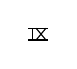
\begin{tikzpicture}[scale=0.05]
  \draw [black] (-2,1.5) to (0,1.5);
          		\draw [black] (-2,-1.5) to (0,-1.5);
		\draw [black] (-1,1.5) to (-1,-1.5);
		\draw [black] (0,1.5) to (2.5,-1.5);
		\draw [black] (0,-1.5) to (1.20,-0.06);
		\draw [black] (1.30,0.06) to (2.5,1.5);
                \draw [black] (0,1.5) to (2.5,1.5);
		\draw [black] (0,-1.5) to (2.5,-1.5);
		\draw [black] (2.5,-1.5) to (3.0,-1.5);
		\draw [black] (2.5,1.5) to (3.0,1.5);
              \end{tikzpicture}}

\newcommand{\IceCream}{	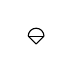
\begin{tikzpicture}[scale=0.05]
	\draw[color = black, fill=none] (2,0) arc(0:180:2);
		\draw [black] (-2,0) to (2,0);
		\draw [black] (-2,0) to (0,-2);
                	\draw [black] (2,0) to (0,-2);
	\end{tikzpicture}}

            
            \newcommand{\Kite}{	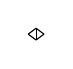
\begin{tikzpicture}[scale=0.05]
              		\draw [black] (-2,0) to (-0,1.5);
		\draw [black] (-2,0) to (-0,-1.5);
                	\draw [black] (2,0) to (0,1.5);
                        \draw [black] (2,0) to (0,-1.5);
                        \draw[black] (0,1.5) to (0,-1.5);\end{tikzpicture}}

\newcommand{\chickenDiag}{	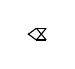
\begin{tikzpicture}[scale=0.05]
		\filldraw [black] (-2,0) circle (2pt);
%		\draw [black] (-2,0) to (-3,0);
%		\filldraw [black] (0,1.5) circle (2pt);
%		\filldraw [black] (0,-1.5) circle (2pt);
%		\filldraw [black] (2.5,1.5) circle (2pt);
%		\filldraw [black] (2.5,-1.5) circle (2pt);
		\draw [black] (-2,0) to (-0,1.5);
		\draw [black] (-2,0) to (-0,-1.5);
		\draw [black] (0,1.5) to (2.5,-1.5);
		\draw [black] (0,-1.5) to (1.20,-0.06);
		\draw [black] (1.30,0.06) to (2.5,1.5);
		\draw [black] (0,1.5) to (2.5,1.5);
		\draw [black] (0,-1.5) to (2.5,-1.5);
	%	\draw [black,thick] (2.5,-1.5) to (3.0,-1.5);
%		\draw [black,thick] (2.5,1.5) to (3.0,1.5);
\end{tikzpicture}}
%%%%%%%%%%%%%%%%%%%%%%%%%%%%%%%%%%%%%%%%%%%%%%%%%%%%%%%%%%%%%%%%%%
\begin{document}
\preprint{IPHT-t23/094, LAPTH-003/24}
\title{\bf Algorithm for differential equations for Feynman integral
  in general dimensions}
\author[]{Leonardo de la Cruz}
\author[]{and Pierre Vanhove}

\affiliation[]{Institut de Physique Theorique, Universit\'e Paris-Saclay,
CEA, CNRS, F-91191 Gif-sur-Yvette Cedex, France}
% e-mail addresses: one for each author, in the same order as the authors
%\keywords{}
 \abstract{
{\bf Draft version \today\ at \thistime}
We present an algorithm for
determining the minimal order differential equations associated to a given
Feynman integral in dimensional or analytic regularisation.  The algorithm is an extension
of the Griffiths-Dwork approach adapted to the twisted differential
associated to Feynman integrals.


We demonstrate the applicability of this algorithm by providing the
inhomogeneous differential equations for the dimensionally regularised
multiloop two-point sunset integrals: up to the 20th loop order for
the all equal mass case, the generic mass case at the two-loop and the
three-loop order. Additionally, we present the Picard-Fuchs operator
for the two-loop three-point ice-cream cone graph, and other two-loop graphs.


We apply as well our algorithm to the dimensionally and analytically regulated Witten diagrams for cosmological correlators of conformally coupled $\phi^4$
  theory in four-dimensional de Sitter space.

}

\maketitle
%\newpage

%%%%%%%%%%%%%%%%%%%%%%%%%%%%%%%%%%%%%%%%%%%%%%%%%%%%%%%%%%%%%%%%%%
\section{Introduction}

Feynman integrals are ubiquitous in various areas of physics, and their accurate calculation, whether analytically or numerically, remains a significant hurdle in advancing our understanding of physical phenomena.
%
In particular, identifying the specific types of special functions required to evaluate Feynman integrals has been an ongoing challenge since the early days of quantum field theory~\cite{Golubeva,Pham} and  continues to be an active research field, with recent contributions from studies such as~\cite{Panzer:2015ida,Duhr:2019wtr,Mizera:2019ose,Travaglini:2022uwo}.\lNote{maybe a review?}


\medskip
By deriving the set of differential operators acting on a Feynman integral one
gets important information about its analytic nature. For instance, 
the differential  operator has real singularities at the position of
 thresholds and pseudo-thresholds, and the order of the differential
operator is connected to the underlying algebraic geometry of the singular locus
of the integrand~\cite{Doran:2023yzu}. Intriguingly, there is  growing evidence suggesting that certain
Feynman integrals correspond to relative period integrals of singular
Calabi--Yau geometries, a connection explored in a number
of studies,
including~\cite{Brown:2009ta,Bloch:2014qca,Bloch:2016izu,Bourjaily:2018ycu,Bourjaily:2019hmc,Bourjaily:2018yfy,Klemm:2019dbm,Bonisch:2020qmm,Bonisch:2021yfw,Bourjaily:2022bwx,Forum:2022lpz,Duhr:2022pch,Frellesvig:2023PM,Pogel:2023zyd}.

It has been remarked that correlation
functions~\cite{Heckelbacher:2022hbq}
and cosmological correlators~\cite{Heckelbacher:2022fbx,Chowdhury:2023arc}
of conformally
coupled $\phi^4$ field in four dimensions can be expressed in term of
flat space Feynman integrals.  The regulation of ultraviolet
divergences lead to integrals in analytical regularisation.

In this work we give an algorithmic procedure for deriving such
differential equations and the inhomogeneous part without having to go through the integral
reduction to master integrals and the construction of a reducible
system of differential equation satisfied by the set of master
integrals.  There are several motivations for short cutting the master
integral reductions. The integration-by-part reduction lead to large
system of master integrals that can obscure the algebraic
geometry underlying the analytic
structure of the Feynman integrals.
A second motivation is the application to
cosmological correlators which give rise to analytic regularisation
for which the commonly used integration by part algorithms are not  developed. 

We work with the regularised parametric representation of a Feynman integral $
I_\Gamma^{\epsilon,\kappa}=\int_{x_i\geq0}  \omega_\Gamma^{\epsilon,\kappa} dx_1\cdots dx_n$ attached to a
graph $\Gamma$ (we refer to 
Section~\ref{sec:parametric} for details)
with
\begin{equation}\label{e:OmegaAnRegIntro}
  \omega^{\epsilon,\kappa}_\Gamma = { \textbf{U}_\Gamma ^{\upnu_1+\cdots+\upnu_n-(L+1)\delta}  \over \textbf{F}_\Gamma ^{\upnu_1+\cdots+\upnu_n-L\delta} }\, \left(\textbf{U}_\Gamma^{L+1}\over \textbf{F}_\Gamma^{L}\right)^{\epsilon} 
  \left(\prod_{i=1}^n \left(x_i \textbf{U}_\Gamma(\underline x)\over
      \textbf{F}_\Gamma(\underline x)\right)^{p_i}\right)^{\kappa} \, \prod_{i=1}^n x_i^{\upnu_i-1} .
\end{equation}
We consider case covering
the dimensional regularisation by working in dimension
$D=2\delta-2\epsilon$ and analytically regularised integral where
propagators are raised to a generalised power depending on $\kappa$.

In the case when $\epsilon=\kappa=0$ and $\delta$ a positive integer, the exponents
in~\eqref{e:OmegaAnRegIntro} are
integers and,
we have a rational differential form. One can use the  Griffiths-Dwork
pole reduction~\cite{Griffiths_1969,Griffith1,Griffith2,Dwork_1962,Dwork_1964} for determining the minimal differential operator (the
Picard-Fuchs operator) associated to a given Feynman
integral~\cite{Bloch:2016izu,Vanhove:2018mto,Lairez:2022zkj}.
In this work we give an extension of the Griffiths-Dwork reduction  algorithms in the case when
$\epsilon\neq0$, $\kappa\neq0$ and where $\delta$ is a positive
integer, for which   we have a twisted differential
form.
%
 This way we
can analyse how the space-time dimension or the analytic regulator  affects the order of the
minimal differential operators.



This paper is organised as follows. 
In Section~\ref{sec:parametric} we review the parametric
representation of Feynman integrals, and sets our notations for the 
dimensionally and analytically regulated integrals in Section~\ref{sec:Twisted}.
In Section~\ref{sec:Red} we
present the algorithmic procedure for deriving the differential
equations. In Section~\ref{sec:griff-dwork-reduct},  we generalise the
Griffiths-Dwork pole reduction to the case of the twisted differential
$\omega_\Gamma^{\epsilon,\kappa}$, and explain in
Section~\ref{sec:deriv-diff-equat} how to use this iteratively to
determine the differential equations. This generalises the algorithm  for the rational differential form cases
used in~\cite{Lairez:2022zkj}. In Section~\ref{sec:oneloop}, we
illustrate the procedure on the case of the dimensionally regulated massless box.
We then consider the Witten cross diagram in (A)dS$_4$ in Section~\ref{sec:WittenCross}.
In
Section~\ref{sec:twoloop}, we derive the $\epsilon$-deformed
differential equation for the two-loop sunset integral for various
mass configurations, the massless double-box and the ice-cream cone
graph. We give a Gr\"obner basis of differential operators for the
analytically regulated
two-loop ice-cream graph entering the cosmology correlator in dS$_4$. In Section~\ref{sec:higherloop}, we give the $\epsilon$-deformed
differential
equation for the all equal mass sunset up to twenty loop orders, for
the three-loop massive sunset.
In Section~\ref{sec:minim-order-diff}
we discuss the question of the minimal order differential operator,
and in Section~\ref{sec:epsilon-dependence} we analyze how the
$\epsilon$ parameter enters the differential
equation. Section~\ref{sec:conclusion} contains a short
conclusion. The Appendix~\ref{sec:bessel} is dedicated to a short
discussion of the derivation of the differential equation using the
Bessel representation with the Creative telescoping algorithm.

%%%%%%%%%%%%%%%%%%%%%%%%%%%%%%%%%%%%%%%%%%%%%%%%%%%%%%%%%%%%%%%%
\section{Twisted differential from regulated Feynman integrals}
\label{sec:parametric}

We will apply our formalism in dimensional regularisation for Feynman integrals and analytic regularisation for Witten diagrams. Their treatment is slightly different so we will consider them separately. 

\subsection{Review of the parametric representation}
We consider the parametric  representation of Feynman
integrals  in $D$ space-time dimensions associated to a graph $\Gamma$ with $n$   internal edges and $L$ loops. Its derivation can be found  in~\cite{nakanishi1971graph,Vanhove:2014wqa,Bogner:2010kv,Weinzierl:2022eaz} for instance. 
%
The differential form associated to a Feynman integral is 
\begin{equation}\label{e:OmegaDef}
	\omega_\Gamma ={ \textbf{U}_\Gamma ^{\nu_1+\cdots+\nu_n-{(L+1)D\over2}}  \over
  \textbf{F}_\Gamma ^{\nu_1+\cdots+\nu_n-{LD\over2}} }\, \prod_{i=1}^n
x_i^{\nu_i-1}; \qquad 	\Omega_\Gamma :=	\omega_\Gamma \, \Omega^{(n)}_0,
\end{equation}
where we have introduced the  canonical differential form on
$\mathbb P^{n-1}$ 
% 
\begin{equation}
	\Omega_0^{(n)}:=  \sum_{i=1}^n (-1)^{i-1} x_i dx_1\wedge \cdots \wedge \widehat{dx_i} \wedge\cdots \wedge dx_n ,
\end{equation}
and where  $\widehat{dx_i}$ means that the term is omitted in the wedge
product. We denote collectively the 
variables 
attached to all edges of
$\Gamma$ as $\underline x:=\{x_i |1\leq i\leq n\}$. 
%
The polynomials $\textbf{U}_\Gamma$ and $\textbf{F}_\Gamma$
associated to  $\Gamma$ are defined as
follows~\cite{nakanishi1971graph,Bogner:2010kv,Weinzierl:2022eaz}.  The {\em first
	Symanzik polynomial} is defined by
\begin{equation}\label{e:Udef}
	{\bf U}_\Gamma (\underline x)= \sum_{\mathsf{T} \in \substack{ \text{Spanning} \\ \text{ trees of } \Gamma}} x_{\mathsf{T}}\,, 
\end{equation}
where the sum is over all the spanning trees $\mathsf{T}$ of $\Gamma$,  i.e.  all subgraphs ${\sf T}$ of $\Gamma$ which contain all
vertices of $\Gamma$ so that the first betti number (i.e. the number
of loop) $b_1(\mathsf{T}) =0$ and the number of connected component
is 
$b_0(\mathsf{T})=1$. The
monomial is the product of the variables not in the spanning tree
$x_{\mathsf{T}} = \prod_{e\notin {\mathsf{T}}} x_e$.  This is a
homogeneous polynomial of 
%$L$ in the edge variables 
$\deg(\textbf{U}_\Gamma(\underline x))=L$.
The {\em second 
	Symanzik polynomial}  $\textbf{F}_\Gamma$ is defined by
\begin{equation}\label{e:VFdef}
	{\bf V}_{\Gamma} (\underline x)= \sum_{\substack{ \text{Spanning} \\ \text{ 2-forests
				of } \Gamma}}s_{\mathsf{F}} x_{\mathsf{F}}
	,\qquad {\bf F}_{\Gamma}(\underline x) = {\bf
		U}_\Gamma(\underline x)\left( \sum_{e \in e(\Gamma)} m_e^2 x_e\right) - {\bf V}_{\Gamma}\,,
\end{equation}
where $x_{\mathsf{F}} =
\prod_{e \notin \mathsf{F}} x_i$ to each spanning 2-forest. A 2-forest
is a disjoint union of two sub-trees $\mathsf{F}=\mathsf{T}_1\cup \mathsf{T}_2$. 
This is an
homogeneous polynomial of  
%$L+1$ in the edge variables
$\deg(\textbf{F}_\Gamma(\underline x))=L+1$.
With the dot denoting the scalar product on $\mathbb R^{1,D-1}$,  we define the invariant of $\mathsf T$ as $s_\mathsf{F} = \sum_{(v_1,v_2) \in \mathsf{F}=\mathsf{T}_1\cup \mathsf{T}_2} p_{v_1}\cdot p_{v_2}$ .
The second Symanzik polynomial carries all dependence on the physical parameters, that is 
the
internal masses and the external kinematics, which we  write as 
\begin{equation}
	\vec m:=\{m_1,\dots,m_n\}, \quad  \vec s:=\{s_\textsf{F} \mid \textsf{F} ~ \textrm{spanning
		2-forests of}~\Gamma\}\, ,	
\end{equation}
respectively.



The differential form~(\ref{e:OmegaDef}) is defined in the middle cohomology $H^{n-1}(\mathbb P^{n-1}\backslash
\{\textbf{U}_\Gamma \textbf{F}_\Gamma=0\})$~\cite{bek,Brown:2009ta}.
The Feynman integral associated with the graph $\Gamma$ is 
given by the integral $  I_\Gamma = \int_{\Delta_n}
\, \Omega_\Gamma$ of the  differential form over
the positive orthant
\begin{equation}\label{e:Deltan}
	\Delta_n:=\{(x_1,\dots,x_n)\in \mathbb P^{n-1}, x_i \geq0 ~\textrm{for}~ 1\leq
	i\leq n\},
\end{equation}

%-----------------------------------------------------------------------
\subsection{Twisted differential forms}\label{sec:Twisted}

The Feynman integral $I_\Gamma$ can diverge  for integer values of $D$ and 
the exponents $\nu_i$, but there is an open subset of
$(D,\nu_1,\dots,\nu_n)\in\mathbb C^{n+1}$ where  the integral
converges,  and the (unique) value of the Feynman integral is  defined by analytic continuation~\cite{Speer}.


We work in dimension $D=2\delta-2\epsilon$ with $\delta\in\mathbb N^*$ and
$\epsilon\in\mathbb R$ and  considers as well that the power of the propagators are shifted from integer values, that is  $\nu_i=\upnu_i
+ p_i \kappa$ with $\{\upnu_1,\dots,\upnu_n,p_1,\dots,p_n\}\in\mathbb Z^{2n}$, so that the 
differential form~(\ref{e:OmegaDef}) becomes the twisted
differential form $\Omega^{\epsilon,\kappa}_\Gamma
=\omega^{\epsilon,\kappa}_\Gamma \Omega_0^{(n)}$ with
\begin{equation}\label{e:OmegaTwistAnaReg}
	\omega^{\epsilon,\kappa}_\Gamma := { \textbf{U}_\Gamma
		^{\upnu_1+\cdots+\upnu_n-(L+1)\delta}  \over \textbf{F}_\Gamma
		^{\upnu_1+\cdots+\upnu_n-L\delta}
	}\,\left(\textbf{U}_\Gamma^{L+1}\over \textbf{F}_\Gamma^L\right)^\epsilon
	\left(\prod_{i=1}^n \left(x_i \textbf{U}_\Gamma(\underline x)\over
	\textbf{F}_\Gamma(\underline x)\right)^{p_i}\right)^{\kappa} \, \prod_{i=1}^n x_i^{\upnu_i-1} \,.
\end{equation}
%
The twists are the $\epsilon$ or $\kappa$-th powers of a homogeneous
degree zero rational functions on $\mathbb
P^{n-1}$.


Notice that we do not assume that $\epsilon$ or $\kappa$ are small numbers.
When $\kappa=0$ we have the parametric representation of a Feynman
integral in dimension regularisation and we will use the short end
notation 
\begin{equation}\label{e:OmegaTwistDimReg}
\omega^\epsilon_\Gamma:=\omega^{\epsilon,0}_\Gamma = { \textbf{U}_\Gamma ^{\nu_1+\cdots+\nu_n-(L+1)\delta}  \over \textbf{F}_\Gamma ^{\nu_1+\cdots+\nu_n-L\delta} }\,
	\left(\textbf{U}_\Gamma^{L+1}\over \textbf{F}_\Gamma^{L}\right)^{\epsilon} \, \prod_{i=1}^n x_i^{\nu_i-1} \, .
\end{equation}
%

\medskip

The differential forms~(\ref{e:OmegaTwistDimReg})
and~(\ref{e:OmegaTwistAnaReg}) are twisted
twisted differential of the kind
studied~\cite{Aomoto1,Aomoto,Aomoto_1982,AomotoBook}.
The
relevance to Feynman integrals was already recognised in these works. 
This has been applied in
e.g.~\cite{Mizera:2017rqa,Frellesvig:2019uqt,Cacciatori:2021nli,Munch:2023ifm,Brunello:2023rpq,Teschke:2024bct}  for
expanding Feynman integrals on the basis of master integrals. In contrast to these works, 
%
we will use
the fact that the twist is given by
the power of the homogeneous degree 0 rational form
which will be essential
in the construction presented in this work.


%%%%%%%%%%%%%%%%%%%%%%%%%%%%%%%%%%%%%%%%%%%%%%%%%%%%%%%%%%%%%%%%%%
\section{Annihilators of Feynman integrals}
\label{sec:Red}
Feynman integrals are holonomic functions of its physical parameters~\cite{Kashiwara:1977nf, Bitoun:2017nre, Smirnov:2010hn,Lee:2013hzt}. This means that Feynman integrals satisfy systems of  (inhomogeneous) partial
differential equations of finite order with respect to its physical
parameters $\vec m$ and $\vec s$.

Let us consider $r$ parameters from the set of internal masses and independent kinematics, $\underline z:=\{z_1,\dots,z_r\} \in \vec m \cup \vec s $. 
%
We seek 
differential operators 
annihilating the differential form $\Omega_\Gamma^{\epsilon,\kappa}$ 
\begin{equation}\label{e:PFOmegaGeneric}
	\left(  \sum_{a_1=0}^{o_1} \sum_{ a_r=0}^{o_r} c_{a_1,\dots,a_r}(\vec m,\vec s,\epsilon,\kappa)\left(\partial\over \partial z_1\right)^{a_1}\cdots\left(\partial
	\over\partial z_r\right)^{a_r}  \right)\Omega_\Gamma^{\epsilon,\kappa}=d\beta^{\epsilon,\kappa}_\Gamma,
\end{equation}
where $c_{a_1,\dots,a_r}(\vec m,\vec s,\epsilon,\kappa)$ are rational functions of the physical
parameters but they are independent of the edge variables $x_1,\dots,x_n$. The inhomogeneous term is a total derivative in $x_i$'s where the only allowed poles are those already present in $\Omega_\Gamma^{\epsilon,\kappa}$~\cite{Lairez:2022zkj}.
%
Because the domain of integration of the Feynman integral does not
depend on the physical parameters, we then deduce
\begin{equation}\label{e:PDEintFeynman}
	\left( \sum_{a_1=0}^{o_1} \sum_{ a_r=0}^{o_r} c_{a_1,\dots,a_r}(\vec m,\vec s,\epsilon,\kappa)\left(\partial\over \partial z_1\right)^{a_1}\cdots\left(\partial
	\over\partial z_r\right)^{a_r}  \right)I^{\epsilon,\kappa}_\Gamma=\mathscr{S}^{\epsilon,\kappa}_\Gamma \, ,
\end{equation}
where $\mathscr{S}^{\epsilon,\kappa}_\Gamma$ is an inhomogeneous term obtained by
integrating $d\beta^{\epsilon,\kappa}_\Gamma$ over the boundary of
orthant~\eqref{e:Deltan}. This is a nontrivial task because one needs
to blow-up the intersections between the graph hypersurface and the
domain of integration so the integral is well
defined~\cite{bek,Brown:2009ta,Bloch:2016izu,muller2014picard}. For
instance, 
Section~3.2 of~\cite{Bloch:2016izu} gives  a detailed derivation of the inhomogeneous term for
the two-loop sunset integral along these lines.

If the integration is done a cycle $\mathcal C$, like the one
defined  by the maximal cut $\mathcal C_{\rm
  max}:=\{|x_1|=\cdots=|x_n|=1\}$,  the resulting integral is
annihilated by the  action of the differential operator~\cite{Vanhove:2018mto}
\begin{equation}
	\left( \sum_{a_1=0}^{o_1} \sum_{ a_r=0}^{o_r} c_{a_1,\dots,a_r}(\vec m,\vec s,\epsilon,\kappa)\left(\partial\over \partial z_1\right)^{a_1}\cdots\left(\partial
	\over\partial z_r\right)^{a_r}  \right)\int_{\mathcal C }\Omega^{\epsilon,\kappa}_\Gamma=0\,.
\end{equation}
%


The ideal  generated by these
differential operators is a differential module (or D-module).  Thus,
differential equations can be obtained by deriving  annihilators  of
$\Omega_\Gamma^{\epsilon,\kappa}$, i.e., partial differential operators that
annihilate  the integrand by acting on the physical parameter and the
edge variables.   The Gel'fand-Kapranov-Zelevinsky (GKZ) formalism provides
a D-module of differential operator acting on the toric generalisation
of the Feynman
integral~\cite{Vanhove:2018mto,delaCruz:2019skx,Klausen:2019hrg,Feng:2019bdx,Klemm:2019dbm,Ananthanarayan:2022ntm,Agostini:2022cgv,
	Munch:2022ouq}.  For obtaining the differential module acting on a
given Feynman integral one needs to restrict the GKZ  D-module which
is an higher non trivial task~\cite{delaCruz:2019skx,Chestnov:2023kww} and its systematic implementation is
still an open problem. In the following sections we present an
algorithmic procedure for deriving the differential equation based on
an extension of the Griffiths-Dwork reduction for twisted differential forms.



%-------------------------------------------------------------------
\subsection{Griffiths-Dwork reduction for twisted differential forms}\label{sec:griff-dwork-reduct}
The    differentiation of $\Omega_\Gamma^{\epsilon,\kappa}$ 
leads  to  expressions of the type 
\begin{multline}\label{e:PDE}
\sum_{\mathsf{a}=a_1+\cdots+a_r\atop
  a_i\geq0}c_{a_1,\dots,a_r}(\vec m,\vec s,\epsilon,\kappa)\left(\partial\over \partial z_1\right)^{a_1}\cdots\left(\partial
  \over\partial z_r\right)^{a_r} \Omega_\Gamma^{\epsilon,\kappa}=\cr
{ \sum_{\mathsf{a}=a_1+\cdots+a_r\atop a_i\geq0}
  c_{a_1,\dots,a_r}(\vec m,\vec s,\epsilon,\kappa)  P^{(a_1,\dots,a_r)}(\underline x)\over \textbf{F}_\Gamma^{\mathsf {a}}}\, \Omega_\Gamma^{\epsilon,\kappa},
\end{multline}
where 
$  P^{(a_1,\dots,a_r)}(\underline x)$ is a
  homogeneous polynomial of degree $(L+1)(a_1+\cdots+a_r)$ in
  the edge variables $\underline x$.
  The sum is over the differential operators of order
  $a_1\geq0 ,\dots, a_r\geq0$ and fixed total order $\mathsf{a}:=a_1+\cdots +a_r$. 
The
  pole order in the second Symanzik polynomial $\textbf{F}_\Gamma$ has increased by
  $\mathsf a$. 
  For deriving~Eq.~\eqref{e:PFOmegaGeneric} one needs to find the
  coefficient $ c_{a_1,\dots,a_r}(\vec m,\vec s,\epsilon,\kappa)$.  From now on we consider the case where
  $\nu_1=\cdots=\nu_r=1$ so that $\nu=n$. The case with $\nu_i\neq1$
  is an immediate generalisation.

  
%-----------------------------------------------------------------------
  \subsubsection{The pole reduction for dimensional
    regularisation}\label{sec:PoleRed}
We give an adaption of the Griffiths-Dwork pole reduction to the case
of the twisted differential form~(\ref{e:OmegaTwistDimReg}) from
dimensional regularisation (i.e. $\kappa=0$ and $\epsilon\neq0$).
The starting point of the algorithm is the reduction of polynomial
$P^{(a_1,\dots,a_r)}(\underline x)$  in the numerator
of~\eqref{e:PDE}
\begin{equation}\label{e:RedF}
	P^{(a_1,\dots,a_r)}(\underline x) = \vec C_{\mathsf{a}}(\underline x)\cdot
	\vec\nabla   \textbf{F}_\Gamma \, ,
      \end{equation}
      where we have introduce the gradient $	\vec\nabla   \textbf{F}_\Gamma :=\left(\partial_{x_1}
      \textbf{F}_\Gamma(\underline x),\dots, \partial_{x_n}
      \textbf{F}_\Gamma(\underline x)\right)$.
%
The components of the size $n$ vector $ \vec C_{\mathsf{a}}(\underline x)$ are homogeneous polynomials of degree
$\mathsf{a}(L+1)-L$ in  $\underline x$ . 
%
 %    
   We generalize the construction by
   Griffiths~\cite{Griffith1,Griffith2} to include the twist factor
   for $\mathsf{a}>1$ 
   \begin{equation}\label{e:betadef}
  \beta^{(a_1,\dots,a_r)}=  \sum_{1\leq i<j\leq n} {x_i
    G_{\mathsf{a}}^j  (\underline x)-x_j
   G_{\mathsf{a}}^i(\underline x)\over
  \textbf{F}_\Gamma^{\mathsf{a}-1}}\, 
 dx_1\wedge \cdots \wedge \widehat{dx_i}\wedge \cdots \wedge\widehat{dx_j}\wedge
  \cdots \wedge dx_n \, .
\end{equation}
To take into account the general dimensional case, we introduce 
the vectors of twisted forms
\begin{equation}
  \label{e:Gdef}
\vec  G_{\mathsf{a}}(\underline x):=   \vec C_{\mathsf{a}} \,\Omega_\Gamma^\epsilon \, ,
\end{equation}
whose components are vectors of homogeneous degree $(\mathsf{a}-1)(L+1)+1-n$. 
Following the same steps as in~\cite{Griffiths_1969}, we have
\begin{multline}
  d\beta_\Gamma^{(a_1,\dots,a_r)}=-  (\mathsf{a}-1) \sum_{1\leq i<j\leq n} {x_i
    G_{\mathsf{a}}^j  (\underline x)-x_j
   G_{\mathsf{a}}^i(\underline x)\over
   \textbf{F}_\Gamma^{\mathsf{a}}}\, d \textbf{F}_\Gamma\wedge
 dx_1\wedge \cdots \wedge \widehat{dx_i}\wedge \cdots \wedge\widehat{dx_j}\wedge
 \cdots \wedge dx_n \cr
+  \sum_{1\leq i<j\leq n} {d(x_i
    G_{\mathsf{a}}^j  (\underline x)-x_j
   G_{\mathsf{a}}^i(\underline x))\over
   \textbf{F}_\Gamma^{\mathsf{a}-1}}\wedge
 dx_1\wedge \cdots \wedge \widehat{dx_i}\wedge \cdots \wedge\widehat{dx_j}\wedge
  \cdots \wedge dx_n  \, .
\end{multline}
Using the homogeneity of $\mathbf{F}_\Gamma$ and the
components of $\vec G_{\mathsf{a}}(\underline x)$ we have
\begin{align}
  \sum_{i=1}^n x_i {\partial\mathbf{F}_\Gamma (\underline x)\over \partial x_i}&=
                                                                  (L+1) \mathbf{F}_\Gamma (\underline x),\cr
   \sum_{i=1}^n x_i {\partial\vec G_{\mathsf{a}}(\underline x)\over \partial x_i}&=
                                                                  ((\mathsf{a}-1)(L+1)+1-n) \vec G_{\mathsf{a}}(\underline x) \,,
\end{align}
we find that 
   \begin{equation}
     d\beta_\Gamma^{(a_1,\dots,a_r)}= (\mathsf{a}-1) {  \vec  G_{\mathsf{a}}
     (\underline x)
\cdot    \vec \nabla\textbf{F}_\Gamma\over
     \textbf{F}_\Gamma^{\mathsf{a}}}\Omega_0^{(n)}-{
\vec\nabla \cdot \vec G_{\mathsf{a}}
     (\underline x)
    \over
   \textbf{F}_\Gamma^{\mathsf{a}-1}}
  \Omega_0^{(n)} \,.
\end{equation}
Using the definition of $\vec  G_{\mathsf{a}}$ in~\eqref{e:Gdef} we
have reduced the pole order  of $ \textbf{F}_\Gamma$ in~\eqref{e:PDE} 
\begin{equation}\label{e:RedG1}
 (\mathsf{a}-1)\left(\partial\over \partial z_1\right)^{a_1}\cdots\left(\partial
  \over\partial z_r\right)^{a_r} \Omega_\Gamma^\epsilon={
\vec\nabla \cdot \vec G_{\mathsf{a}}
     (\underline x)
    \over
  \textbf{F}_\Gamma^{\mathsf{a}-1}}
  \Omega_0^{(n)}+d\beta_\Gamma^{(a_1,\dots,a_r)}.
\end{equation}
%
We expand the first term in the right-hand-side
\begin{equation}
  \vec\nabla \cdot \vec G_{\mathsf{a}}(\underline x)=  \vec\nabla \cdot \vec C_{\mathsf{a}}(\underline x) {\textbf{U}_\Gamma^{\lambda_U}\over
  \textbf{F}_\Gamma^{\lambda_F}} 
+
  \vec C_{\mathsf{a}}(\underline x) \cdot\vec\nabla  \left(   {\textbf{U}_\Gamma^{\lambda_U}\over
  \textbf{F}_\Gamma^{\lambda_F}} \right),
\end{equation}
where we have defined
\begin{equation}\label{e:powerUFDef}
  \lambda_U=n-(L+1)(\delta-\epsilon), \qquad 
  \lambda_F=n-L(\delta-\epsilon).
  \end{equation}
%
The second term in this equation can be evaluated using 
\begin{align}
  \vec C_{\mathsf{a}}(\underline x)\cdot \vec\nabla \left(\mathbf{U}_\Gamma^{\lambda_U}\over
\mathbf{F}_\Gamma^{\lambda_F}\right)&=\left(\lambda_U \vec
C_{\mathsf{a}}\cdot \vec\nabla \log\mathbf{U}_\Gamma -{\lambda_F} \vec
C_{\mathsf{a}}\cdot \vec\nabla \log \mathbf{F}_\Gamma\right) {\mathbf{U}_\Gamma^{\lambda_U}\over
\mathbf{F}_\Gamma^{\lambda_F}} \cr
&=\left[-{\lambda_F}{
    P^{(a_1,\dots,a_r)}(\underline x)\over
  \mathbf{F}_\Gamma}   
+
 \lambda_U \vec
C_{\mathsf{a}}\cdot \vec\nabla \log\mathbf{U}_\Gamma \right] {\mathbf{U}_\Gamma^{\lambda_U}\over
	\mathbf{F}_\Gamma^{\lambda_F}}\,,
\end{align}
where we have used Eq.~\eqref{e:RedF} in the second equality. Therefore, 
\begin{equation}
	\label{e:Pred}
\left(\partial\over \partial z_1\right)^{a_1}\cdots\left(\partial
  \over\partial z_r\right)^{a_r} \Omega_\Gamma^\epsilon={
\vec\nabla \cdot \vec C_{\mathsf{a}}
     (\underline x)
+ \lambda_U \vec
    C_{\mathsf{a}}\cdot\vec\nabla\log\mathbf{U}_\Gamma\over \left(\mathsf{a}-1+\lambda_F\right)\,\textbf{F}_\Gamma^{\mathsf{a}-1}}
  \Omega_\Gamma^\epsilon
+{  1\over \mathsf{a}-1+\lambda_F} d\beta_\Gamma^{(a_1,\dots,a_r)}.
\end{equation}
%
This expression involves the $\vec
    C_{\mathsf{a}}\cdot\vec\nabla\log\mathbf{U}_\Gamma$ which has a
    pole in $\mathbf{U}_\Gamma$. We then perform a second reduction by demanding that
    \begin{equation}
      \label{e:RedU}
      \vec
    C_{\mathsf{a}}(\underline x)\cdot\vec\nabla \mathbf{U}_\Gamma =
    c_{\mathsf{a}}(\underline x) \, \mathbf{U}_\Gamma \, ,
    \end{equation}
where $ c_{\mathsf{a}}(\underline x)$ is a homogeneous polynomial of
degree $(\mathsf{a}-1)(L+1)$. This is equivalent to the computation of
syzygies of $\text{Jac}( \mathbf
U_\Gamma):=\langle \vec\nabla \textbf{U}_\Gamma(\underline x)\rangle$. Indeed,  using the homogeneity of $\mathbf{U}_\Gamma$ we can rewrite the previous equation as 
\begin{equation}
 \left( L   \vec
C_{\mathsf{a}}(\underline x) -
c_{\mathsf{a}}(\underline x) \vec{x} \right) \, \cdot\vec\nabla
\mathbf{U}_\Gamma =0\, ,
\end{equation}
which are examples of syzygies of the Jacobian of $\mathbf U_\Gamma$. Using this reduction in eq.~\eqref{e:Pred} leads to
% 
\begin{equation}\label{e:RedFinal}
\left(\partial\over \partial z_1\right)^{a_1}\cdots\left(\partial
  \over\partial z_r\right)^{a_r} \Omega_\Gamma^\epsilon={
M^{(a_1,\dots,a_r)}
     (\underline x)
\over \textbf{F}_\Gamma^{\mathsf{a}-1}}\Omega_\Gamma^\epsilon
+{  \mathsf{a}-1\over \mathsf{a}+n-L(\delta-\epsilon)} d\beta_\Gamma^{(a_1,\dots,a_r)}
\end{equation}
with the numerator given by the polynomial of homogeneous degree $(\mathsf{a}-1)(L+1)$
\begin{equation}
  \label{e:Mdimregfinal}
  M^{(a_1,\dots,a_r)}(\underline x):={\vec\nabla \cdot \vec C_{\mathsf{a}}
     (\underline x)
+ \lambda_U\, 
    c_{\mathsf{a}}(\underline x)\over \mathsf{a}-1+\lambda_F },
\end{equation}
with $\lambda_U$ and $\lambda_F$ the powers of the $\textbf{U}_\Gamma$
and the $\textbf{F}_\Gamma$ polynomials respectively given in~\eqref{e:powerUFDef}.
%




To perform this pole reduction, 
 we have to solve the linear system
\begin{equation}\label{e:sysCFU}
   \left\{\begin{array}{@{}l@{}}
\vec C_{\mathsf{a}} (\underline x) \cdot \vec \nabla \textbf{F}_\Gamma
            =    P^{(a_1,\dots,a_r)}(\underline x)\\
\vec C_{\mathsf{a}} (\underline x)\cdot\vec \nabla\textbf{U}_\Gamma= c_{{\mathsf{a}}}(\underline x) \textbf{U}_\Gamma 
  \end{array}\right.\,,
\end{equation}
for determining the coefficients of $\vec C_{\mathsf{a}}(\underline
x)$ and $c_{\mathsf{a}}(\underline x)$.
%
The system~\eqref{e:sysCFU} has a solution when its rank is positive.
We have a linear system of the $n$ components of $\vec C_{\mathsf{a}}(\underline
x) $ which are homogeneous polynomial of degree $\deg(C)=\deg( P^{(a_1,\dots,a_r)})-L $ in
$\underline x$ and  $ c_{{\mathsf{a}}}(\underline x) $ which is a polynomial of
homogeneous degree $\deg(C)-1$.   Since the number of coefficients of
a homogeneous polynomial of degree $d$ in $n$ variables is
$\binom{d+n-1}{d}$,  the system has
\begin{equation}\label{e:nvars}
n \binom{\deg( P^{(a_1,\dots,a_r)})-L+n-1}{\deg( P^{(a_1,\dots,a_r)})-L}+\binom{\deg( P^{(a_1,\dots,a_r)})-L+n-2}{\deg( P^{(a_1,\dots,a_r)})-L-1}
\end{equation} unknown variables for
\begin{equation}\label{e:nequ}
\binom{\deg( P^{(a_1,\dots,a_r)})+n-1}{\deg( P^{(a_1,\dots,a_r)})}+\binom{\deg( P^{(a_1,\dots,a_r)})+n-2}{\deg( P^{(a_1,\dots,a_r)})-1}
\end{equation}
equations.
%
%
Since the $\deg(P^{(a_1,\dots,a_r)})=\mathsf{a}(L+1)$, the rank of the system~\eqref{e:sysCFU} is
  \begin{align}
    \label{e:Rank}
    \textrm{rank}&=\eqref{e:nvars}-\eqref{e:nequ}\\
\nonumber    &=n \binom{(L+1)(\mathsf{a}-1)+n
               }{(L+1) (\mathsf{a}-1)+1}+\binom{(L+1)(\mathsf{a}-1)+n-1}{(L+1) (\mathsf{a}-1)}\cr
             \nonumber    &
                              -\binom{(L+1) \mathsf{a}+n-1}{(L+1) \mathsf{a}}-\binom{(L+1) \mathsf{a}+n-2}{(L+1) \mathsf{a}-1}
  \end{align}
For fixed values of the loop order $L$
and the number of edges $n$ there is always a value of the
number of derivative $\mathsf{a}$ such that the system has
positive rank.

A few comments are in order. In practice for Feynman integrals,   the polynomial $ P^{(a_1,\dots,a_r)}(\underline x)$ is not a generic
homogeneous polynomial so the number of equations is smaller or equal than~\eqref{e:nequ}.
%
We remark that this way of solving the linear system includes implicitly the
freedom given by the syzygies of $\textrm{Jac}(\textbf{F}_\Gamma)
 :=\langle \vec\nabla \textbf{F}_\Gamma(\underline x)\rangle$ and
$\textrm{Jac}(\textbf{U}_\Gamma)$ since they belong to
the kernel of equation~\eqref{e:RedF} and~\eqref{e:RedU}
respectively.\footnote{It was noticed in~\cite{Lairez:2022zkj} that in
  the rational case only the first order sygyzies are needed to take
  into account the non-isolated singularities of Feynman integrals.}
%
%
%
One important property of that reduction is that the differential form $\beta_\Gamma^{(a_1,\dots,a_n)}$ is that it
does not have poles that are not poles of $\textbf{F}_\Gamma$ which is
guaranteed by the construction. We refer
to Section~3 of~\cite{Lairez:2022zkj} for a discussion of the pole constraints.
%
%
%-----------------------------------------------------------------------
  \subsubsection{The pole reduction for analytic
    regularisation}\label{sec:PoleRedAn}
We give an adaption of the Griffiths-Dwork pole reduction to the case
of the twisted differential form~(\ref{e:OmegaTwistAnaReg})  from
analytical regularisation. Since most of the steps are similar to the
one presented in the previous section we only give the main equations.

As before we reduce the  polynomial
$P^{(a_1,\dots,a_r)}(\underline x)$ in the Jacobian of
$\textbf{F}_\Gamma$ using eq.~(\ref{e:RedF}) and introduce the
differential forms~\eqref{e:betadef}
$\beta_\Gamma^{(a_1,\dots,a_r)}$  and the vector of differential forms $\vec
G_{\mathsf{a}}(\underline x)$ as in eq.~\eqref{e:Gdef}, leading to the
pole reduction eq.~\eqref{e:RedG1}.
Because the twist is different the expansion of the 
right-hand-side  (recall that $D=2\delta-2\epsilon$)
\begin{equation}
  \vec\nabla \cdot \vec G_{\mathsf{a}}(\underline x)=  \vec\nabla \cdot \vec C_{\mathsf{a}}(\underline x) { \textbf{U}_\Gamma ^{\lambda_U}  \over \textbf{F}_\Gamma ^{\lambda_F} }\,
  Q(\underline x)^\kappa
+
  \vec C_{\mathsf{a}}(\underline x) \cdot\vec\nabla  \left({ \textbf{U}_\Gamma ^{\lambda_U}  \over \textbf{F}_\Gamma ^{\lambda_F} }\,
  Q(\underline x)^\kappa \right) ,
\end{equation}
where we have set (we have assumed that $\upnu_1=\cdots=\upnu_n=1$ the
generic case of integer values is an easy generalisation)
\begin{equation}
  Q(\underline x):=\prod_{i=1}^n x_i^{p_i}   
\end{equation}
and defined the powers of the various polynomials by
\begin{equation}
  \label{e:powerUFQDef}
  \lambda_U= n-(L+1)(\delta-\epsilon)+\kappa\sum_{i=1}^n p_i, \qquad
  \lambda_F= n-L(\delta-\epsilon)+\kappa\sum_{i=1}^n p_i, \qquad
  \lambda_Q  = \kappa\,.
\end{equation}
%
This is  evaluated using 
\begin{equation}
  \vec C_{\mathsf{a}}(\underline x)\cdot \vec\nabla
  \left(\mathbf{U}_\Gamma^{\lambda_U}Q(\underline x)^\kappa\over
\mathbf{F}_\Gamma^{\lambda_F}\right)=\Big(\lambda_U \vec
C_{\mathsf{a}}\cdot \vec\nabla \log\mathbf{U}_\Gamma -\lambda_F \vec
C_{\mathsf{a}}\cdot \vec\nabla \log \mathbf{F}_\Gamma+\lambda_Q \vec
C_{\mathsf{a}}\cdot\vec\nabla \log Q(\underline                             x)\Big)
                            {\mathbf{U}_\Gamma^{\lambda_U}Q(\underline x)^\kappa\over
\mathbf{F}_\Gamma^{\lambda_F}} .
\end{equation}
so that
\begin{multline}
	\label{e:PredAnReg}
\left(\partial\over \partial z_1\right)^{a_1}\cdots\left(\partial
  \over\partial z_r\right)^{a_r} \Omega_\Gamma^{\epsilon,\kappa}={
\vec\nabla \cdot \vec C_{\mathsf{a}}
     (\underline x)
+  \lambda_U \vec
    C_{\mathsf{a}}\cdot\vec\nabla\log\mathbf{U}_\Gamma+\lambda_Q \vec
    C_{\mathsf{a}}\cdot\vec\nabla\log Q(\underline x)\over
    \left(\mathsf{a}-1+\lambda_F\right)\,\textbf{F}_\Gamma^{\mathsf{a}-1}}\,
  \Omega_\Gamma^{\epsilon,\kappa}\cr
+{  1 \over \mathsf{a}-1+\lambda_F} d\beta_\Gamma^{(a_1,\dots,a_r)}.
\end{multline}
%
This time we need to reduce the pole in $\mathbf{U}_\Gamma$ from  the term $\vec
    C_{\mathsf{a}}\cdot\vec\nabla\log\mathbf{U}_\Gamma$ and the new
    pole in $1/x_i$ from the twisted propagators.
    As before we do impose the following conditions
\begin{equation}\label{e:sysCFUAnReg}
   \left\{\begin{array}{@{}l@{}}
\vec C_{\mathsf{a}} (\underline x) \cdot \vec \nabla \textbf{F}_\Gamma
            =    P^{(a_1,\dots,a_r)}(\underline x)\\
\vec C_{\mathsf{a}} (\underline x)\cdot\vec \nabla\textbf{U}_\Gamma=
            c_{{\mathsf{a}}}(\underline x) \textbf{U}_\Gamma \\
            \vec C_{\mathsf{a}} (\underline x)\cdot\vec \nabla
            Q(\underline x)=
            q_{{\mathsf{a}}}(\underline x) Q(\underline x)
  \end{array}\right.\,,
\end{equation}
leading to the pole  reduction in eq.~\eqref{e:PDE} 
% 
\begin{equation}\label{e:RedFinalAnReg}
\left(\partial\over \partial z_1\right)^{a_1}\cdots\left(\partial
  \over\partial z_r\right)^{a_r} \Omega_\Gamma^\epsilon={
M^{(a_1,\dots,a_r)}
     (\underline x)
\over \textbf{F}_\Gamma^{\mathsf{a}-1}}\Omega_\Gamma^\epsilon
+{  1\over \mathsf{a}-1+\lambda_F} d\beta_\Gamma^{(a_1,\dots,a_r)}
\end{equation}
with the numerator given by the polynomial of homogeneous degree $(\mathsf{a}-1)(L+1)$
\begin{equation}
  \label{e:MfinalAnReg}
  M^{(a_1,\dots,a_r)}(\underline x):={
\vec\nabla \cdot \vec C_{\mathsf{a}}
     (\underline x)
+  \lambda_U
    c_{\mathsf{a}}(\underline x)+\lambda_Q q_{\mathsf{a}}(\underline x)\over
    \mathsf{a}-1+\lambda_F}.
\end{equation}
%


%----------------------------------------------------------------------
\subsubsection{Determination of the differential equations}
\label{sec:deriv-diff-equat}


We turn to the derivation of the differential
equation~\eqref{e:PFOmegaGeneric}  by iterating the generalized
Griffiths-Dwork reduction given in the previous sections. We present an algorithm for a derivation of
a linear ordinary differential equation with respect to a single
variable differentiation $z$ (either an internal mass, or a kinematic
variable or a scaling parameter as used
in~\cite{Lairez:2022zkj,Doran:2023yzu}) so that $r=1$ and $\mathsf{a}=a_1$. The generalisation to the
many variables case is immediate.

We are seeking the differential operator 
\begin{equation}\label{e:PFgeneric}
  \mathscr{L}_\Gamma^{\epsilon,\kappa}=\sum_{\mathsf{a}=0}^{N(\Gamma,\epsilon,\kappa)}
  c_{\mathsf{a}}x(\vec m,\vec s,\epsilon,\kappa) \left(d\over dt\right)^{\mathsf{a}}
\end{equation}
with $c_{\mathsf{a}}(\vec m,\vec s,\epsilon,\kappa)$ polynomials in the internal masses
$\vec m$  and the (independent) kinematic variables $\vec s$  and the
regulators $\epsilon$  and $\kappa$, such that
\begin{equation}
     \mathscr{L}_\Gamma^{\epsilon,\kappa} \Omega_\Gamma^{\epsilon,\kappa}= d\beta^{\epsilon,\kappa}_\Gamma.
   \end{equation}
%
Holonomicity of Feynman integrals gives an upper bound on the order of the Picard-Fuchs operator $N(\Gamma,\epsilon,\kappa)$, which is  determined by
 the number of master
integrals. Let $N(\Gamma,\epsilon,\kappa)$  be the starting order of the
reduction.  We then apply the results of Sections~\ref{sec:PoleRed}
or~\ref{sec:PoleRedAn} so that
%
\begin{equation}\label{e:step1}
\left(d\over dt\right)^{N(\Gamma,\epsilon,\kappa)} \Omega_\Gamma^\epsilon= {M^{
      N(\Gamma,\epsilon,\kappa)}(\underline x)\over
    \textbf{F}_\Gamma^{N(\Gamma,\epsilon)-1}
  } \,\Omega_\Gamma^{\epsilon,\kappa}+ d\beta_\Gamma^{N(\Gamma,\epsilon,\kappa)}  
\end{equation}
%
The next step we add the lowest-order derivative

\begin{multline}\label{e:step2}
\left[\left(d\over dt\right)^{N(\Gamma,\epsilon,\kappa)}
  +q_{N(\Gamma,\epsilon)-1}(t,\epsilon,\kappa) \left(d\over dt\right)^{N(\Gamma,\epsilon,\kappa)-1}\right] \Omega_\Gamma^{\epsilon,\kappa}\cr= {M^{
      N(\Gamma,\epsilon,\kappa)}(\underline x)+q_{N(\Gamma,\epsilon,\kappa)-1}(t,\epsilon,\kappa)
    P^{N(\Gamma,\epsilon,\kappa)-1}(\underline x) \over
    \textbf{F}_\Gamma^{N(\Gamma,\epsilon,\kappa)-1}
  }\,\Omega_\Gamma^{\epsilon,\kappa}+ d\beta_\Gamma^{N(\Gamma,\epsilon,\kappa)}\, ,  
\end{multline}
where the rational coefficient
$q_{N(\Gamma,\epsilon,\kappa)-1}(t,\epsilon)=c_{N(\Gamma,\epsilon,\kappa)-1}(t,\epsilon)/c_{N(\Gamma,\epsilon,\kappa)}(t,\epsilon)$
is an unknown rational function of $t$ and  the regulators $\epsilon$
and $\kappa$. 
The polynomial $ P^{N(\Gamma,\epsilon,\kappa)-1}(\underline x) $
is the numerator factor obtained by taking the $N(\Gamma,\epsilon,\kappa)-1$
derivative of the differential form.

We then apply the reduction of Section~\ref{sec:PoleRed} or~\ref{sec:PoleRedAn} to
the polynomial in the numerator
$M^{
      N(\Gamma,\epsilon,\kappa)}(\underline x)+q_{N(\Gamma,\epsilon,\kappa)-1}(t,\epsilon)
    P^{N(\Gamma,\epsilon,\kappa)-1}(\underline x)$.
The resolution of the
system~\eqref{e:sysCFU} determines the  rational coefficient
$q_{N(\Gamma,\epsilon,\kappa)-1}(t,\epsilon)$ and
$M^{N(\Gamma,\epsilon,\kappa)-1}(x)$ computed using~(\ref{e:MfinalAnReg}). One
iterates the reduction until the power of  the second Symanzik
polynomial $\textbf{F}_\Gamma$ is $n-L-1$ so
that
\begin{equation}\label{e:stepfinal}
\left[\left(d\over dt\right)^{N(\Gamma,\epsilon,\kappa)}
  +\sum_{\mathsf{a}=1}^{N(\Gamma,\epsilon,\kappa)-1}
  {c_{N(\Gamma,\epsilon,\kappa)-\mathsf{a}}(t,\epsilon)\over c_{N(\Gamma,\epsilon,\kappa)}(t,\epsilon)} \left(d\over dt\right)^{N(\Gamma,\epsilon,\kappa)-\mathsf{a}}\right] \Omega_\Gamma^{\epsilon,\kappa}=M^{0}\,\Omega_\Gamma^{\epsilon,\kappa}+ d\beta_\Gamma^{\epsilon ,\kappa}
\end{equation}
where $M^0$ is of degree 0 so that we
\begin{equation}
  q_0(t,\epsilon,\kappa)=  {c_{0}(t,\epsilon,\kappa)\over
    c_{N(\Gamma,\epsilon,\kappa)}(t,\epsilon,\kappa)}= -M^0  .
\end{equation}
The inhomogeneous term  $\beta_\Gamma^{\epsilon,\kappa} $ is the sum of the
$\beta^{\mathsf{a}}$ with $1\leq
\mathsf{a}\leq N(\Gamma,\epsilon,\kappa)$
contributions with their multiplicative factor as given
in~\eqref{e:Pred}
\begin{equation}
  \label{e:betaGamma}
  \beta_\Gamma^{\epsilon,\kappa}= \sum_{1\leq i<j\leq n} (x_i B^j_\Gamma- x_j B^i_\Gamma) \,
  dx_1\wedge \cdots \wedge \widehat{dx_i}\wedge \cdots \wedge\widehat{dx_j}\wedge
  \cdots \wedge dx_n 
\end{equation}
with
\begin{equation}
  \label{e:BetaGamma}
  \vec B_\Gamma:=\left(\sum_{\mathsf{a}=1}^{N(\Gamma,\epsilon,\kappa)} {
      \vec C_{\mathsf{a}} (\underline x) \over
   ( \mathsf{a}-1+n-L(\delta-\epsilon))\mathbf{F}_\Gamma^{\mathsf{a}-1}}\right) \,\omega_\Gamma^\epsilon ,
\end{equation}
which is a vector of degree of homogeneity $1-n$ in the edge variables
$\underline x$.
Since $d\beta_\Gamma^{\epsilon,\kappa}= -\vec\nabla\cdot \vec B_\Gamma\,
\Omega_0^{(n)}$, from~\eqref{e:stepfinal} we have the ordinary
differential equation satisfied by the integrand of the Feynman
integral
\begin{equation}\label{e:stepfinalode}
\left[\left(d\over dt\right)^{N(\Gamma,\epsilon,\kappa)}
  +\sum_{r=0}^{N(\Gamma,\epsilon,\kappa)-1}
  {c_{N(\Gamma,\epsilon,\kappa)-r}(t,\epsilon)\over c_{N(\Gamma,\epsilon,\kappa)}(t,\epsilon)} \left(d\over dt\right)^{N(\Gamma,\epsilon,\kappa)-r}\right] \omega_\Gamma^\epsilon =-\vec\nabla\cdot \vec B_\Gamma\,.
\end{equation}


\medskip
 
 Let us comment on how to determine the order of the Picard-Fuchs operators. An upper bound on the order can be computed
 from the number of master integrals.
 The number of master
integrals  can be computed from the Euler
characteristic of complement of the graph polynomial~\cite{Bitoun:2017nre} or counting the
critical points of the Euler representation of the integral in
projective
space~\cite{Lee:2013hzt,Cacciatori:2021nli}
or~\cite{Mastrolia:2018uzb,Frellesvig:2019uqt} (see~\cite{Agostini:2022cgv} for
a discussion of the relation between the different ways of computing the number of master
integrals). On the other hand, determining the minimal order is a
difficult question. Our pragmatical approach is to increase the order
starting from 
lower orders until the system~\eqref{e:sysCFU} has a solution, which is
the spirit of the Griffiths-Dwork reduction applied to Feynman
integrals in~\cite{Muller-Stach:2011qkg}.

In practice, for determining the minimal order it is enough to run the step of the
Griffiths-Dwork reduction for fixed generic numerical values for the physical
parameters (the internal masses and kinematic
parameters), because all the reduction amounts to solve a linear system in the projective space of
the edge parameters $\underline x$. This allows to determine the smallest order for which the
algorithm closes to give a differential operator.

In general, the Griffiths-Dwork algorithm does not automatically
leads to an irreducible Picard-Fuchs differential operator.
The factorisation of an linear ordinary
differential operator can be done with the {\tt DFactor} routine from
{\tt Maple} up to the order 4 for generic parameters~\cite{PutSinger,vanHoeij}, and to any
orders for linear  ordinary
differential operators with numerical coefficients
using the {\tt facto} algorithm in {\tt
	sagemath}~\cite{chyzak2022symbolic,goyer2021sage}.


 In the rational case $\epsilon=\kappa=0$, it was noticed
in~\cite{Bloch:2013tra,Bloch:2016izu,Bloch:2014qca,Lairez:2022zkj} that the order of the minimal differential operator is
smaller than the number of irreducible master integrals.
When the regulator take integer values the minimal order is smaller
than the number of master integrals. 
In the various cases studied below,
we will see that the order of the minimal differential operator can saturates
the upper bound given by the number of masters for generic values of
the regulators  $\epsilon$  and $\kappa$. 
This will
      be discussed further in Section~\ref{sec:minim-order-diff}.


%%%%%%%%%%%%%%%%%%%%%%%%%%%%%%%%%%%%%%%%%%%%%%%%%%%%%%%%%%%%%%%%%
\section{One-loop examples}\label{sec:oneloop}
We start in Section~\ref{sec:box} with the simple example of the
massless  one-loop box in dimensional regularisation, which will serve
as an illustration of where the main features of the algorithm emerge.

We then work out a Gr\"obner basis of differential operators
associated with the Cross Witten diagram for conformally coupled 
$\phi^4$  in  four dimensional  de Sitter space. It was shown
 in~\cite{Heckelbacher:2022fbx,Heckelbacher:2022hbq}  that the
 cosmological correlators of conformally coupled $\phi^4$ can be organised  as dimensionally regulated flat space Feynman integrals in position
space. Because of the measure of integration in (anti)-de Sitter the
resulting integrals fall into the category of the analytic
continuation of Section~\ref{sec:Twisted}. 


%------------------------------------------------------------------------
\subsection{The massless box graph in dimensional regularisation}\label{sec:box}
\begin{figure}[ht]
	\centering
	\begin{tikzpicture}
		\draw[dashed](-1,-1)--(-1.3,-1.3);
		\draw[dashed](1,-1)--(1.3,-1.3);
		\draw[dashed](1,1)--(1.3,1.3);
		\draw[dashed](-1,1)--(-1.3,1.3);
		\draw[dashed, thick](-1,-1)--(-1.0,1.0)--(1.0,1.0)--(1.0,-1.0)--cycle;
		\node[text width=0.5cm, text centered ] at (-1.2,0) {$1$};
		\node[text width=0.5cm, text centered ] at (0,-1.3) {$2$};
		\node[text width=0.5cm, text centered ] at (1.2, 0) {$3$};
		\node[text width=0.5cm, text centered ] at (0,1.3) {$4$};
		\node[text width=0.5cm, text centered ] at (-1.5,1.5){$k_1$};
		\node[text width=0.5cm, text centered ] at (1.5,1.5){$k_2$};
		\node[text width=0.5cm, text centered ] at (1.5,-1.5){$k_3$};
		\node[text width=0.5cm, text centered ] at (-1.5,-1.5){$k_4$};
	\end{tikzpicture} 
\caption{The box  graph with massless external and internal states.
  The external momenta are $k_i$ with $k_1+\cdots+k_4=0$. The
          labels of the graph give the index of the edge variable $x_i$. }\label{fig:box}
\end{figure}
\begin{comment}
\begin{figure}[h]\centering
	\begin{tikzpicture}[scale=0.6]
		\filldraw [color = black, fill=none, dashed] (0,0) circle (2cm);
		\draw [black,dashed] (1.414,1.414) to (2.25,2.25);
		\draw [black,dashed] (-1.414,1.414) to (-2.25,2.25);
		\draw [black,dashed] (1.414,-1.414) to (2.25,-2.25);
		\draw [black,dashed] (-1.414,-1.414) to (-2.25,-2.25);
	\end{tikzpicture}
	\caption{The box  graph with massless external and internal states.}\label{fig:box}
\end{figure}
\end{comment}

The first example we consider is the so-called on-shell massless box. We define the usual Mandelstam invariants as $t=(k_1+k_3)^2$, $s=(k_1+k_2)^2$.  The graph polynomials are given by
\begin{equation}
	\label{e:Boxgraphpolynomials}
	\textbf{U}_{\Box}=\sum_{i=1}^4 x_i,\qquad
	\textbf{F}_{\Box}(s,t)=-t x_2x_4-sx_1x_3 \, .
\end{equation}
The twisted differential in $D=4-2\epsilon$ in the projective
space $\mathbb P^3$
\begin{equation}\label{e:OmegaBox}
	\Omega_\Box^\epsilon=   {1\over \textbf{F}_{\Box}(s,t)^2
	}\left(\textbf{U}_{\Box}^2\over \textbf{F}_{\Box}(s,t)\right)^\epsilon\,\Omega_0^{(4)} \, .
\end{equation}
This is a single scale function depending only on the ratio
$X=t/s$ of the kinematic invariant so we scale the integral obtaining
$\tilde \Omega_\Box^\epsilon(X)=(-s)^{2+\epsilon} \Omega_\Box^\epsilon(s,X s)$ .
%
The application of the procedure given in
Section~\ref{sec:deriv-diff-equat} needs only to start at the first
order. Computing the derivative with respect to $X$ we obtain 
%
\begin{equation}
P  ^{(1)}= (2+\epsilon) x_2 x_4 \, , 
\end{equation}
which we will reduce with respect to the $\text{Jac}(\mathbf F_\Box)=\langle \partial_{x_1}\textbf{F}_\Box=-x_3, \partial_{x_2}\textbf{F}_\Box= -x_4 X, \partial_{x_3}\textbf{F}_\Box=-x_1, -X x_2  \rangle$. The  vector  $\vec C_{1}(\underline x)$ has components 
\begin{equation}
C^i_{1}(\underline x)= \sum_{e \in m_{2,4}} \lambda^i_e x^e,	
\end{equation}
where $m_{i,j}$ denote the set of exponent vectors of degree $i$ in $j$ variables. Since $\deg(C^i_{1}(\underline x))=2$, $\deg (c_1(\underline x))=1$, i.e., $c_1(\underline x)=\sum_{e\in m_{1,4}} q_e x^e$. Hence the linear system becomes
%
\begin{equation}\label{e:sysCFU-Box}
	\left\{\begin{array}{@{}l@{}}
\sum_i \sum_{e \in m_{2,4}} \lambda^i_e x^e \text{Jac}_i(\mathbf F_\Box) 
		=    (2+\epsilon) x_2 x_4\\
\sum_i\sum_{e \in m_{2,4}} \lambda^i_e x^e \text{Jac}_i(\mathbf U_\Box) = \sum_{e\in m_{1,4}} q_e x^e \textbf{U}_\Box 
	\end{array}\right.\,,
\end{equation}
which leads to 
%
\begin{equation}
	c_0= \frac{1+X+\epsilon }{X(X+1)}.
\end{equation}
We then derive
\begin{equation}\label{e:PFBox}
	\mathscr{L}_\Box^\epsilon= (X+1) X {d\over dX}+(1+X+\epsilon)  \,.
\end{equation}
In this simple case the algorithm only requires one iteration. 
The inhomogeneous term reads
\begin{equation}\label{e:SourceBox}
	\mathscr{S}_\Box^\epsilon=\frac{(\epsilon +1)\Gamma (-\epsilon -1)^2 }{\Gamma
		(-2 \epsilon )}  \, \left( (-s)^{-1-\epsilon }+(-t)^{-\epsilon -1}\right) \, .
\end{equation}
This simple example illustrates the general procedure as we will see with more loops. In general the system of equations is dense. As usual when one encounters dense  systems, finite field methods are the way to go~\cite{Peraro:2019svx}.
%-------------------------------------------------------------------------
\subsection{The Cross Witten diagram in AdS$_4$ in dimensional regularisation}\label{sec:WittenCross}
\begin{figure}[ht]
	\centering
	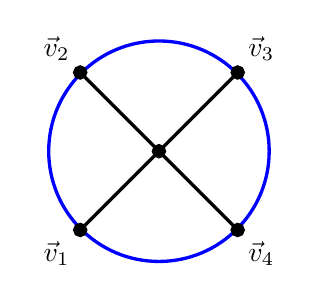
\begin{tikzpicture}[very thick]
		\path [draw](-1,-1) --(1,1);
		\path [draw](-1,1) --(1,-1);
		\draw[blue] circle (1.4cm);
		\coordinate (A) at (0,0);   \filldraw (A) circle (2.pt);
		\coordinate (B) at (-1,1);   \filldraw (B) circle (2.pt);
		\coordinate (C) at (-1,-1);   \filldraw (C) circle (2.pt);
		\coordinate (D) at (1,1);   \filldraw (D) circle (2.pt);
		\coordinate (E) at (1,-1);   \filldraw (E) circle (2.pt);
		\node[text width=0.5cm, text centered ] at
                (-1.3,1.3){$\vec v_2$};
		\node[text width=0.5cm, text centered ] at
                (-1.3,-1.3){$\vec v_1$};
		\node[text width=0.5cm, text centered ] at
                (1.3,-1.3){$\vec v_4$};
		\node[text width=0.5cm, text centered ] at
                (1.3,1.3){$\vec v_3$};
	\end{tikzpicture}
  \caption{Witten Cross diagram, between four states on
	boundary of $dS_4$. }
\label{fig:cross}
	\end{figure}
\begin{comment}
 \begin{figure}[ht]
                \centering
                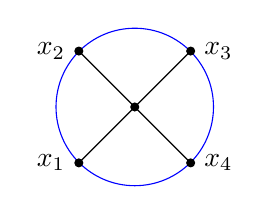
\begin{tikzpicture}[baseline=(z)]
                        \begin{feynman}[inline=(z)]
                                \tikzfeynmanset{every vertex=dot}
                                \vertex (z);
                                \vertex [above left=0.71cm and 0.71cm of z, label=180:$x_2$] (x2);
                                \vertex [below left=0.71cm and 0.71cm of z, label=180:$x_1$] (x1);
                                \vertex [above right=0.71cm and 0.71cm of z, label=0:$x_3$] (x3);
                                \vertex [below right=0.71cm and 0.71cm of z, label=0:$x_4$] (x4);
                                \tikzfeynmanset{every vertex={empty dot,minimum size=0mm}}
                                \diagram* {
                                        (x2)--(z),
                                        (x1)--(z),
                                        (x3)--(z),
                                        (x4)--(z),
                                };
                        \end{feynman}
                        \begin{pgfonlayer}{bg}
                                \draw[blue] (z) circle (1cm);
                        \end{pgfonlayer}
                \end{tikzpicture}
                \caption{Witten Cross diagram, between four states on
                  boundary of $dS_4$. }
                \label{fig:cross}
        \end{figure}

\end{comment}
The dimensionally regulated Witten cross diagram of Fig.~\ref{fig:cross} considered in
Section~4.1 of~\cite{Heckelbacher:2022fbx} is given by the integral
over the bulk point $X$

\begin{equation}
       \mathcal{ W}_0^{1,4-4\varepsilon}(\zeta,\bar\zeta)=\frac12\frac{\zeta\bar\zeta}{(v_{12}v_{34})^2}\int_{\mathbb{R}^4}\frac{d^{4-4\varepsilon}X}{\|X\|^2\|X-u_1\|^{2(1-4\varepsilon)}\|X-u_{\zeta}\|^2}\,.
\end{equation}
with the vectors  $u_1=(1,0,0,0)$ and 
$u_{\zeta}=\left(\frac{\zeta+\bar\zeta}{2},\frac{\zeta-\bar\zeta}{2i},0,0\right)$ where $\zeta$  and $\bar\zeta$ parameterise the cross ratios $\zeta\bar\zeta=v_{12}^2v_{34}^2/(v_{14}^2v_{23}^2)$ and
  $(1-\zeta)(1-\bar\zeta)=v_{13}^2v_{24}^2 /(v_{14}^2 v_{23}^2)$
  defined by the position on the boundary of (A)dS$_4$.

The parametric representation is given by
$
  I_\times(\zeta,\bar\zeta)= \int_{\Delta_3}   \Omega_\times^{2\varepsilon,-4\varepsilon}(\zeta,\bar\zeta)
$ the integration over the twisted differential form
\begin{equation}
  \Omega_\times^{2\varepsilon,-4\varepsilon}(\zeta,\bar\zeta)={\pi^{2-2\varepsilon}\Gamma(1-2\varepsilon)\over\Gamma(1-4\varepsilon)} {1\over \textbf{U}_\times
    \textbf{F}_\times (\zeta,\bar\zeta)} \left(
    \textbf{F}_\times (\zeta,\bar\zeta)^{2}\over  x_2^{4}\right)^\varepsilon  \, \Omega_0^{(3)}
\end{equation}
over the domain $\Delta_3=\{x_i\geq0, 1\leq i\leq 3\}$ and with the graph polynomials
\begin{equation}
  \textbf{U}_\times= x_1+x_2+x_3,  \qquad \textbf{F}_\times (\zeta,\bar\zeta)= x_1x_2+
  \zeta\bar\zeta x_1x_3+ (1-\zeta)(1-\bar\zeta)x_2x_3  .
\end{equation}
We can apply the algorithm to the case of the analytic regularisation
of Section~\ref{sec:PoleRedAn} 
with $\delta=2$, $\epsilon=\kappa=2\varepsilon$, $(p_1,p_2,p_3)=(0,-2,0)$
to find the following set of  differential operators
acting on $I_\times(\zeta,\bar\zeta)$
\begin{multline}
  \mathscr{L}_{\times,1}= (\zeta -1) (\zeta -\bar\zeta) \zeta ^2{\partial^2\over\partial\zeta^2}  +
   \left(\zeta (3 \zeta -\bar\zeta-2)-2\varepsilon  \left(\zeta ^2+\zeta 
   \bar\zeta-2 \bar\zeta\right) \right) \zeta {\partial\over\partial\zeta}\cr+(2 \varepsilon -1) \left(2 \varepsilon  (\zeta +\bar\zeta)-\zeta ^2\right)
\end{multline}
and
\begin{equation}
  \mathscr{L}_{\times,2}= (\zeta -1)\zeta\bar\zeta{\partial\over\partial\zeta}  +
   (\bar\zeta -1)\zeta\bar\zeta{\partial\over\partial\bar\zeta}+\zeta\bar\zeta-2\varepsilon(\zeta+\bar\zeta).
 \end{equation}
 We have checked  with
  the command {\tt OreGroebnerBasis} from the package {\tt
    HolonomicFunctions}~\cite{Koutchan} that
they form a Gr\"obner basis with respect to the lexicographical
ordering $\zeta,\bar\zeta$.

 The algorithm determines the boundary terms 
 such that
 \begin{equation}
   \mathscr{L}_{\times,r}    \left( {1\over \textbf{U}_\times
    \textbf{F}_\times (\zeta,\bar\zeta)} \left(
    \textbf{F}_\times (\zeta,\bar\zeta)^{2}\over
    x_2^{4}\right)^\varepsilon \right)+ \vec\nabla\cdot\vec B_{\times,r}=0.
\qquad r=1,2.
\end{equation}
%
Details are provided in the  attached {\tt Mathematica} worksheet. 




The algorithm gives all the information for computing the
inhomogeneous term of the differential equations acting on the Feynman
integrals. The inhomogeneous term  is given by the  integration of
$\vec\nabla\cdot \vec B_\times$ in~\eqref{e:BetaGamma}  over the
positive orthant. Performing this integration is an highly non-trivial
task for several reasons. A first reason is that the integral of $\vec B_r$
over the domain $\Delta_3$ diverges.
Since these components still
depend on undetermined variables  after having solved the linear systems from the
Griffiths-Dwork reduction, one can make some choice of so that the
restriction of $\vec B_{\times,r}$ to the boundary of the domain of integration
is well defined. Still one needs to regulate the integrals over the
remaining edges variables  to get a finite
result.
Even such a simple case shows that evaluating the
inhomogeneous term is not an easy task, which will not carry for most
of the case studied in this paper. 


%%%%%%%%%%%%%%%%%%%%%%%%%%%%%%%%%%%%%%%%%%%%%%%%%%%%%%%%%%%%%%%
\section{Two-loop examples}\label{sec:twoloop}
%
In this section we apply the algorithm to  the case of dimensionally
 regulated two loop integrals. We derive the $\epsilon$-deformation of
the all equal mass sunset integral in Section~\ref{sec:2sunset1mass}, the general mass configuration
sunset integral in Section~\ref{sec:2sunset3mass}, the two point kite
integral in Section~\ref{sec:kite}, the ice-cream cone
graph in Section~\ref{sec:ice-cream}, the non-planar roast chicken
graph in Section~\ref{sec:chicken} and the four points planar
and non planar boxes~\ref{sec:doubleboxes}. We conclude in  Section~\ref{sec:Wittenicecream}
with the ice-cream cone graph in  analytic regularisation in four
dimensions, which enters the two-loop correction to cosmological
correlators of  conformally coupled $\phi^4$  in  de
 Sitter space~\cite{Chowdhury:2023arc}.
%----------------------------------------------------------------------
\subsection{The two-point  two-loop sunset graph}
\label{sec:two-loop-case}
	\begin{figure}[ht]
		\centering
		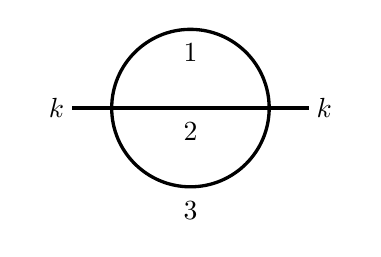
\begin{tikzpicture}
			%\draw[step=1cm,black,very thin] (-1.9,-1.9) grid (1.9,1.9);
			\draw [very thick] (0,1)circle (1);
			\draw[very thick](-1.5,1)--(1.5,1);
			\node[text width=0.5cm, text centered ] at (0,0.7) {$2$};
			\node[text width=0.5cm, text centered ] at (0,1.7) {$1$};
			\node[text width=0.5cm, text centered ] at (0,-0.3) {$3$};
			\node[text width=0.5cm, text centered ] at
                        (-1.7,1.0) {$k$};
                        	\node[text width=0.5cm, text centered ] at (1.7,1.0) {$k$};
		\end{tikzpicture} 
		\caption{The two-loop sunset graph.  The
          labels of the graph give the index of the edge variable $x_i$.}
		  \label{fig:sunset2loop}
	\end{figure}
%
We now turn to the two-loop sunset and shows how to adapt the
Griffiths-Dwork reduction used in~\cite{Bloch:2016izu,Lairez:2022zkj} to the $\epsilon$
dependent integrand. For the two-loop case the differential
Eq.~\eqref{e:OmegaTwistDimReg}, setting $t=k^2$, is
\begin{equation}\label{e:OmegaSunset}
  \Omega_{\su}^{\epsilon}(t)={1\over
    \textbf{F}_2(t)}\left(\textbf{U}_2^3\over \textbf{F}_2(t)^2\right)^\epsilon  \,\Omega_0^{(3)}
\end{equation}
with the graph polynomials 
\begin{align}
 \textbf{U}_2&=x_1x_2+x_1x_3+x_2x_3,\cr
  \textbf{F}_2(t)&=-t x_1x_2x_3 + (m_1^2x_1+m_2^2x_2+m_3^2x_3) \textbf{U}_2.
\end{align}
%
The twisted differential form $\Omega_\su^{\epsilon}$ is defined on the
complement of the sunset elliptic curve $\mathbf{F}_2(t)=0$.
%
We discuss the equal mass and the general case separately.
% Let us start with the equal mass case.
We apply the algorithm by starting to seek an operator of second order which enough for the equal mass case, but for the
three-mass case we find that the minimal order is four, in
agreement with previous results~\cite{Caffo:1998du,Remiddi:2013joa,Adams:2013nia}.

%----------------------------------------------------------------------
\subsubsection{The all equal mass case}\label{sec:2sunset1mass}
We derive the Picard-Fuchs equation satisfied by the two-loop all
equal mass in general dimensions. 
We  start with at $\mathsf{a}=2$ finding
\begin{equation}
 \left(d\over dt\right)^2
 \Omega_{\su}^{\epsilon}(t,\epsilon)={\Gamma(3+2\epsilon)\over\Gamma(1+2\epsilon)} {(x_1x_2x_3)^2\over \textbf{F}_2(t)^3}
 \left(\textbf{U}_2^3\over \textbf{F}_2(t)^2\right)^\epsilon  \Omega_0^{(3)} ,
\end{equation}
from which we can extract $P^{(2)}=2 (\epsilon +1) (2 \epsilon +1)(x_1x_2x_3)^2$. 
%
Accordingly, we label the unknowns with the upper index so $S^{(k)}$ indicates the $k$-th reduction. We then  perform the Jacobian reduction of $P^{(2)}$ as
\begin{equation}\label{e:reduc}
  2 (\epsilon +1) (2 \epsilon +1)\,  (x_1x_2x_3)^2= \sum_{i=1}^3 
  \sum_{e\in m_{4,3}}\lambda^{(2),i}_{e} x^e \text{Jac}_i  (\mathbf{F}_2(t)) \,,
\end{equation}
%
where we have written explicitly the components of $\vec{C}^{(2)}$ as $C^{(2)}_i=\sum_{e\in m_{4,3}}\lambda^{(2),i}_{e} x^e$.
We have to solve the following equation for the coefficients $\lambda_e^{(2)}$ coupled to the equations generated by
\begin{equation}\label{e:C2red}
\sum_{i=1}^3 
\sum_{e\in m_{4,3}}\lambda^{(2),i}_{e} x^e \text{Jac}_i(\mathbf U_2) = \sum_{e\in m_{3,3}} q^{(2)}_e x^e \textbf{U}_2 \,, 
%
\end{equation}
where $c^{(2)}=\sum_{e\in m_{3,3}} q^{(2)}_e x^e$ is an unknown homogeneous degree 3 polynomial
in $\underline x$.
%
The unknowns will be fully determined at the end of  algorithm. For this case, 
the differential form given in eq.~\eqref{e:betadef} reads
%
 \begin{multline}
 	\label{eq:beta-equalmass-sunset}
   \beta_\su^\epsilon=   {x_2  C_3^{(2)}-x_3  C_2^{(2)}\over
     \textbf{F}_2(t)^2} \left(\textbf{U}_2^3\over \textbf{F}_2(t)^2\right)^\epsilon dx_1+   {x_3  C_1^{(2)}-x_1 C_3^{(2)}\over
     \textbf{F}_2(t)^2} \left(\textbf{U}_2^3\over \textbf{F}_2(t)^2\right)^\epsilon dx_2\cr
   +  {x_1  C_2^{(2)}-x_2  C_1^{(2)}\over
    \textbf{F}_2(t)^2} \left(\textbf{U}_2^3\over \textbf{F}_2(t)^2\right)^\epsilon dx_3, 
 \end{multline}
which leads to 
%
\begin{multline}
 (2+2\epsilon)\left(d\over dt\right)^2
  \Omega_{\su}^{\epsilon}(t,\epsilon)=
 \left({\sum_{i=1}^3 \partial_i C_i^{(2)}\over
     \textbf{F}_2(t)^{2}}+3\epsilon{\sum_{i=1}^3 C_i^{(2)}\partial_i
     \log \textbf{U}_2\over \textbf{F}_2(t)^{2}}\right)\cr \times\left(\textbf{U}_2^3\over \textbf{F}_2(t)^2\right)^\epsilon \Omega_0^{(3)}-d(2\beta_\su^\epsilon).
\end{multline}
%
Therefore using eq.\eqref{e:Mdimregfinal}, we define
\begin{equation}
  \label{e:M2}
  M^{(2)}:={\sum_{i=1}^3 \partial^i  C_i^{(2)}+3\epsilon
    c^{(2)}\over 2+2\epsilon} \,, 
\end{equation}
leading to reduction of pole
\begin{equation}
 \left(d\over dt\right)^2
  \Omega_{\su}^{\epsilon}(t,\epsilon)=
{M^{(2)}\over
     \textbf{F}_2^{2}}\left(\textbf{U}_2^3\over \textbf{F}_2(t)^2\right)^\epsilon \Omega_0^{(3)}+d\beta_\su^\epsilon \, ,
 \end{equation}
where we have used~\eqref{e:C2red}.
%
We now add the first derivative with an unknown rational coefficient $q_1(t,\epsilon)$
\begin{multline}
 \left(d\over dt\right)^2
  \Omega_{\su}^{\epsilon}(t,\epsilon) +q_1(t,\epsilon) \left(d\over dt\right)
  \Omega_{\su}^{\epsilon}(t,\epsilon) =
{M^{(1)}\over
     \textbf{F}_2(t)^{2}}\left(\textbf{U}_2^3\over \textbf{F}_2(t)^2\right)^\epsilon \Omega_0+d\beta_\su^\epsilon \, , 
 \end{multline}
where $M^{(1)}:=M^{(2)}+q_1(t,\epsilon) x_1x_2x_3(1+2\epsilon)$.
 We then reduce the pole by writing
 \begin{equation}\label{e:M2red}
   M^{(1)}= \sum_{i=1}^3
   C_i^{(1)} \partial^i \textbf{F}_2(t) \,, 
 \end{equation}
 where $ C_i^{(1)}$ are unknown homogeneous degree 1.
Thus
\begin{equation}
 \left(d\over dt\right)^2
  \Omega_{\su}^{\epsilon}(t,\epsilon) +q_1(t,\epsilon) \left(d\over dt\right)
  \Omega_{\su}^{\epsilon}(t,\epsilon) =
{ \sum_{i=1}^3
   C_i^{(1)} \partial^i \textbf{F}_2(t)\over
     \textbf{F}_2(t)^{2}}\left(\textbf{U}_2^3\over \textbf{F}_2(t)^2\right)^\epsilon \Omega_0+d\beta_\su^\epsilon
 \end{equation}
%
The last step to compute the Picard-Fuchs operator is to derive the constant term, which must reduce the poler order of the right-hand-side of this equation. We thus impose
\begin{equation}\label{e:c0}
  \sum_{i=1}^3C_i^{(1)}\partial^i \textbf{F}_2(t)+ q_0(t,\epsilon) \textbf{F}_2 (t) =0.
\end{equation}
%
Solving all the equations needed for the pole reduction lead
to the unique solution for the coefficients $q_1$ and $q_0$. 
We have the solutions
\begin{align}
  q_1(t,\epsilon)&=\frac{\left(3 t^2-10 t-9\right) \epsilon }{(t-9) (t-1) t}+\frac{3 t^2-20 t+9}{(t-9) (t-1)
   t}\cr
  q_0(t,\epsilon)&=\frac{\epsilon ^2 (2 t+2)}{(t-9) (t-1) t}+\frac{\epsilon  (3 t-5)}{(t-9) (t-1)
   t}+\frac{t-3}{(t-9) (t-1) t} \, ,
\end{align}
leading to the $\epsilon$ dependent \lNote{nomenclature} differential operator
\begin{multline}
  \label{e:PF2sunset1massepsilon}
     \mathscr{L}^{(2),\epsilon,1-mass}_\su ={d\over dt}\left( t(t-1)(t-9)
       {d\over dt}\right)+(t-3)\cr+\epsilon\left((3t^2-10t-9) {d\over
         dt}+3t-5\right)
     +\epsilon^2 2(t+1).
\end{multline}
%
Collecting the inhomogeneous contributions into the vector
\begin{equation}
  \vec B_\su^\epsilon=\sum_{\mathsf{a}=1}^2 {\vec C_{\mathsf{a}}\over
    (\mathsf{a}+2\epsilon)\textbf{F}_\su(t)^{\mathsf{a}-1}}\, \Omega_\su^\epsilon
\end{equation}
one can check that the action of this differential operator on
$\Omega_{\su}^\epsilon(t)$ is
\begin{equation}
      \mathscr{L}^{(2),\epsilon,1-mass}_\su
      \Omega_{\su}^\epsilon(t)+\vec\nabla \cdot\vec B_\su^\epsilon=0
    \end{equation}
as it should be from the general considerations of Section~\ref{sec:deriv-diff-equat}.


\medskip
From the solutions, we can compute the  inhomogeneous term is given by evaluating the integral 
\begin{equation}
  \mathscr{S}_\su^\epsilon
  =-\int_{\Delta_3} \vec\nabla\cdot\vec B^\epsilon_\su.
\end{equation}
%
Because the denominator of $ B^\epsilon_\su$ has a pole at the coordinate
point $[1:0:0]$, $[0:1:0]$ and $[0:0:1]$ one needs to consider the
blow-up  of the domain of integration $\Delta_3$. This is done by inserting a small
$\mathbb P^1$ of radius $\rho$ (see eq.~(3.47) of~\cite{Bloch:2016izu})
\begin{equation}
    \mathscr{S}_\su^\epsilon=\lim_{\rho\to0} \sum_{i=1}^3
    \int_{\partial\tilde\Delta_3|_{x_i=0}} \sum_{1\leq j\neq i\leq 3}
    (B^\epsilon_\su)_j dx_j
\end{equation}
A computation identical to the one performed in~\cite{Bloch:2016izu} leads to
\begin{equation}
 \mathscr{S}_\su^\epsilon=  -6 \, {\Gamma(1+\epsilon)^2\over \Gamma(1+2\epsilon)} \, . 
\end{equation}
The piece of order $\epsilon^0$ reproduces the Picard-Fuchs operator
for the two-loop all equal-mass sunset in $D=2$ given
in~\cite{Bloch:2013tra,Bloch:2013tra,Vanhove:2014wqa,Bonisch:2020qmm,Pogel:2022vat}.

%----------------------------------------------------------------------
\subsubsection{The different mass case}\label{sec:2sunset3mass}

For the non equal mass case the order of the differential equation is
4 with the following $\epsilon$ expansion
\begin{equation}
     \mathscr{L}^{\epsilon}_\su =   \mathscr{L}^{(1)}_1
     \mathscr{L}^{(2)}_1    \mathscr{L}^{3-mass}_\su +\epsilon
     \mathscr{L}^{(3)}_4+\epsilon^2  \mathscr{L}^{(4)}_3+\epsilon^3
     \mathscr{L}^{(5)}_2+ \epsilon^4 \mathscr{L}^{(6)}_1 +\epsilon^5
    \mathscr{L}^{(7)}_0
   \end{equation} 
   where $ \mathscr{L}^{(r)}_m$  are irreducible differential operator
   of  order $m$ and $\mathscr{L}^{3-mass}_\su$ is the differential
   operator for the three-mass two-loop sunset integral in two
   dimensions. This differential equation reproduces the one 
   derived~\cite{Remiddi:2013joa,Remiddi:2016gno}.
%
The $\epsilon$ deformation does not change the non-apparent
singularities of the differential operator as can be seen from the
coefficient of the highest order term
\begin{multline}
  \mathscr{L}^{\epsilon}_\su \Big\vert_{(d/dt)^4}= t^3\prod_{i=1}^4 (t-
  \mu_i^2) \Big(-\left(2 \epsilon +5\right) t^{2}-2
    \left(m_{1}^{2}+m_{2}^{2}+m_{3}^{2}\right) \left(1+2 \epsilon
    \right) t \cr+ \left(7+6 \epsilon \right)\prod_{i=1}^4 \mu_i
\Big)  \, , 
\end{multline}
where $\mu_i=\{m_1+m_2+m_3,-m_1+m_2+m_3,m_1-m_2+m_3,m_1+m_2-m_3\}$ are
the thresholds.  The $\epsilon$ deformation is only affecting the
apparent singularities, since the $\epsilon$ factor
in~\eqref{e:OmegaSunset} does not change the nature of the singular
locus which is still given by the same elliptic curve as in the
$\epsilon=0$ case.
   
Its action on the Feynman integral is given by 
\begin{equation}
     \mathscr{L}^{\epsilon}_\su  I_\su^\epsilon(\underline
     m,t,\epsilon)=\mathscr{S}^\epsilon_\su(\vec m,t,\epsilon) 
   \end{equation}
   with the source term
   \begin{equation}
     \mathscr{S}(\vec m,t,\epsilon)=\frac{c_{23}(t,\epsilon)\Gamma (\epsilon +1)^2}{ (m_{2} m_{3})^{2 \epsilon}\Gamma (1+2\epsilon)}+\frac{c_{13}(t,\epsilon)\Gamma (\epsilon +1)^2}{ (m_{1} m_{3})^{2 \epsilon }\Gamma (1+2
   \epsilon)}+\frac{c_{12}(t,\epsilon)\Gamma (\epsilon +1)^2}{ (m_{1} m_{2})^{2 \epsilon }\Gamma (1+2
   \epsilon )} \, , 
\end{equation}
where $c_{12}(t,\epsilon)$, $c_{13}(t,\epsilon)$ and
$c_{23}(t,\epsilon)$ are polynomials of degrees 4,2 in $t$ and
$\epsilon$, respectively. The results are provided on the {\tt
  SageMath} worksheet \href{Sunset-Twoloop-3mass-Epsilon.ipynb}{Sunset-Twoloop-3mass-Epsilon.ipynb}
%
Expanding in powers of $\epsilon$ , we have
%
\begin{equation}
    \mathscr{S}(\vec m,t,\epsilon)=\mathscr{S}^0(\vec m,t)
    +\left(c^{(1)}_0(\vec m)+
    \sum_{i=1}^3  c^{(1)}_i(\vec m)\log(m_i)\right)\,  \epsilon+O(\epsilon^2)
\end{equation}
with  the leading term given by
   \begin{equation}
   \mathscr{S}^0(\vec m,t)=60 t^{4}+56\left( m_{1}^{2}+ m_{2}^{2}+
     m_{3}^{2}\right) t^{3}
   -308 \prod_{i=1}^4 \mu_i.
 \end{equation}
For $\epsilon=0$ the two-loop sunset integral satisfies  the
differential equation~\cite{Adams:2013nia,Bloch:2016izu}
\begin{equation}
  \mathscr{L}^{3-mass}_\su f_\su^{(0)}(t)= s_0(\vec m,t)+ \sum_{i=1}^3
  s_i(\vec m,t)\log(m_i^2)  
\end{equation}
with 
\begin{align}
  s_0(\vec m,t)&:=18 t^{4}-24\left(m_{1}^{2}m_{2}^{2}+
       m_{3}^{2}\right) t^{3}-4\left( m_{1}^{4}+m_2^4+m_3^4+10(
       m_{1}^{2} m_{2}^{2}+ m_{1}^{2}
       m_{3}^{2}+m_{2}^{2}
       m_{3}^{2})\right) t^{2}\cr
       &+8
       \left(m_{1}^{2}+m_{2}^{2}+m_{3}^{2}\right)\prod_{i=1}^4\mu_i
       t +2 \prod_{i=1}^4\mu_i^2 \cr
  s_1(\vec m,t)&=\left(4 m_{1}^{2}-2 m_{2}^{2}-2 m_{3}^{2}\right)
       t^{3}+\left(-12 m_{1}^{4}+14 m_{1}^{2} m_{2}^{2}+14 m_{1}^{2}
       m_{3}^{2}+6 m_{2}^{4}-28 m_{2}^{2} m_{3}^{2}+6 m_{3}^{4}\right)
       t^{2}\cr
       &+\Big(12 m_{1}^{6}-22 m_{1}^{4} m_{2}^{2}-22 m_{1}^{4} m_{3}^{2}+16 m_{1}^{2} m_{2}^{4}+16 m_{1}^{2} m_{3}^{4}-6 m_{2}^{6}+6 m_{2}^{4} m_{3}^{2}+6 m_{2}^{2} m_{3}^{4}\cr&-6 m_{3}^{6}\Big) t-2 \left(2 m_{1}^{4}-m_{1}^{2} m_{2}^{2}-m_{1}^{2} m_{3}^{2}-m_{2}^{4}+2 m_{2}^{2} m_{3}^{2}-m_{3}^{4}\right) \prod_{i=1}^4\mu_i\cr
       s_2(\vec m,t)&=\left(-2 m_{1}^{2}+4 m_{2}^{2}-2 m_{3}^{2}\right)
            t^{3}+\left(6 m_{1}^{4}+14 m_{1}^{2} m_{2}^{2}-28
            m_{1}^{2} m_{3}^{2}-12 m_{2}^{4}+14 m_{2}^{2} m_{3}^{2}+6
            m_{3}^{4}\right) t^{2}\cr
            &+\Big(-6 m_{1}^{6}+16 m_{1}^{4} m_{2}^{2}+6 m_{1}^{4} m_{3}^{2}-22 m_{1}^{2} m_{2}^{4}+6 m_{1}^{2} m_{3}^{4}+12 m_{2}^{6}-22 m_{2}^{4} m_{3}^{2}+16 m_{2}^{2} m_{3}^{4}\cr&-6 m_{3}^{6}\Big) t +2 \left(m_{1}^{4}+m_{1}^{2} m_{2}^{2}-2 m_{1}^{2} m_{3}^{2}-2 m_{2}^{4}+m_{2}^{2} m_{3}^{2}+m_{3}^{4}\right) \prod_{i=1}^4\mu_i
\cr
            s_3(\vec m,t)&=-s_1-s_2.
\end{align}
It can be checked that 
\begin{equation}
  \mathscr{S}^0(\vec m,t)=   \mathscr{L}^{(1)}_1
     \mathscr{L}^{(2)}_1    \mathscr{L}^{3-mass}_\su  f_\su^{(0)}(t).
\end{equation}
The logarithmic dependence on the masses arise at the order $\epsilon$ 
 and
 \begin{align}
&     c^{(1)}_0(\vec m)=114 t^{4}+168\left(m_{1}^{2}+ m_{2}^{2}+ m_{3}^{2}\right)
  t^{3}+\Big(-552 (m_{1}^{4}+m_2^4+m_3^4)\cr&+1136 (m_{1}^{2} m_{2}^{2}+
    m_{1}^{2} m_{3}^{2}+ m_{2}^{2} m_{3}^{2})\Big) t^{2}-64
  \left(m_{1}^{2}+m_{2}^{2}+m_{3}^{2}\right) \prod_{i=1}^4\mu_i t +14 \prod_{i=1}^4\mu_i^2\\
& c^{(1)}_1(m_1,m_2,m_3)=-80 t^{4}-\left( 88 m_{1}^{2}+ 68 m_{2}^{2}+68 m_{3}^{2}\right)
 t^{3}+\Big(360 m_{1}^{4}-780 m_{1}^{2} m_{2}^{2}-780 m_{1}^{2}
   m_{3}^{2}\cr&+436 m_{2}^{4}-904 m_{2}^{2} m_{3}^{2}+436
   m_{3}^{4}\Big) t^{2}+\Big(-136 m_{1}^{6}+324 m_{1}^{4}
   m_{2}^{2}+324 m_{1}^{4} m_{3}^{2}-256 m_{1}^{2} m_{2}^{4}\cr&-256
   m_{1}^{2} m_{3}^{4}+68 m_{2}^{6}-68 m_{2}^{4} m_{3}^{2}-68
   m_{2}^{2} m_{3}^{4}+68 m_{3}^{6}\Big) t -28   \prod_{i=1}^4\mu_i\cr&\times\Big(2 m_{1}^{4}-m_{1}^{2} m_{2}^{2}-m_{1}^{2} m_{3}^{2}-m_{2}^{4}+2 m_{2}^{2} m_{3}^{2}-m_{3}^{4}\Big) 
\end{align}
with $c^{(1)}_2(m_1,m_2,m_3)=c^{(1)}_1(m_2,m_1,m_3)$ and $c^{(1)}_3(m_1,m_2,m_3)=c^{(1)}_1(m_3,m_2,m_1)$.
and $c^{(1)}_1(\vec m)+c_2^{(1)}(\vec m)+c_3^{(1)}(\vec m)=4
\mathscr{S}^0(\vec m,t)$.
%-----------------------------------------------------------------------
      \subsection{The two-point one-mass kite}\label{sec:kite}
\begin{figure}[h]
	\centering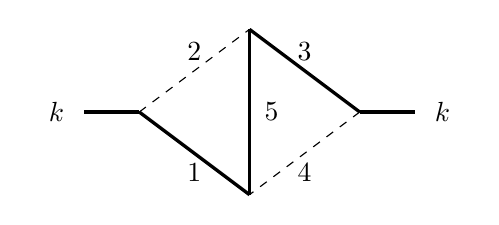
\begin{tikzpicture}[scale=0.7]
		\draw [black, very thick] (-2,0) to (-3,0);
		\draw [black, very thick] (2,0) to (3,0);
		\draw [black, dashed] (-2,0) to (-0,1.5);
		\draw [black, very thick] (-2,0) to (-0,-1.5);
		\draw [black, very thick] (2,0) to (0,1.5);
		\draw [black, dashed] (2,0) to (0,-1.5);
		\draw[black, very thick] (0,1.5) to (0,-1.5);
		\node[text width=0.5cm, text centered ] at (-1.,1.1) {$2$};
		\node[text width=0.5cm, text centered ] at (-1.,-1.1) {$1$};
		\node[text width=0.5cm, text centered ] at (1.,1.1) {$3$};
		\node[text width=0.5cm, text centered ] at (1.,-1.1) {$4$};
		\node[text width=0.5cm, text centered ] at (0.4,0.) {$5$};
		\node[text width=0.5cm, text centered ] at (-3.5,0.0)
                {$k$};
                	\node[text width=0.5cm, text centered ] at (3.5,0.0) {$k$};
	\end{tikzpicture}
	\caption{Special two-point Kite. Dashed lines are massless
          propagators and solid lines are massive propagators. The
          labels of the graph give the index of the edge variable $x_i$.}\label{fig:kite1mass}
\end{figure}
We consider the two points  Kite graph with three massive propagators and
          two massless propagators
\begin{equation}
	\mathbf U_{\Kite} =(x_1+x_2) (x_3+x_4)+(x_1+x_2+x_3+x_4) x_5,
\end{equation}
\begin{multline}
\mathbf F _{\Kite}(m^2,p^2)=k^2 (x_1 x_2 x_3 x_4\sum_{i=1}^4 x_i^{-1}+(x_1+x_4)(x_2+ x_3) x_5)
-m^2 (x_1+x_3+x_5) 	\mathbf U_{\Kite} 
\end{multline}
Now setting $k^2=X m^2$ we have  single scale problem and now set $m=1$
\begin{equation}
  \Omega_{\Kite}^\epsilon=   {\mathbf U_{\Kite}^{5-3\delta}\over
    \mathbf F_{\Kite}(1,X)^{5-2\delta}}\left(\mathbf U_{\Kite}^3\over
    \mathbf F_{\Kite}^2\right)^\epsilon \Omega^{(0)}_5.
\end{equation}

It was shown
in~\cite{Broadhurst:1987ei,Adams:2016xah,Lairez:2022zkj} that the two point Kite graph with generic masses satisfies a
first order differential equation in four dimensions.


The integrand of the Feynman integral is the twisted differential form

\begin{equation}
\Omega_{\Kite} ={	\mathbf U_{\Kite}^{5-3\delta} \over \mathbf (F _{\Kite}(X))^{5-2\delta}}\,\left(	\mathbf U_{\Kite}^3\over \mathbf F _{\Kite}(X)^2\right)^\epsilon\,\Omega^{(0)}_5.
\end{equation}

 \begin{equation}
	\label{eq:Kite}
	\mathscr{L}^\epsilon_{\Kite}=X(X-1){d\over dX} +X-1+(1+X)\epsilon
\end{equation}



%-----------------------------------------------------------------------
\subsection{The three-point ice-cream cone graph}\label{sec:ice-cream}

\begin{figure}[h]
	\centering
	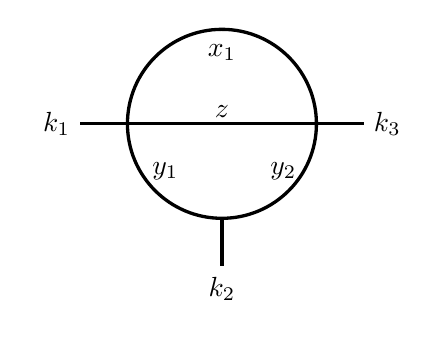
\begin{tikzpicture}[scale=0.6]
		\filldraw [color = black, fill=none, very thick] (0,0) circle (2cm);
	\draw [black,very thick] (-2,0) to (2,0);
	\draw [black,very thick] (-2,0) to (-3,0);
	\draw [black,very thick] (2,0) to (3,0);
	\draw [black,very thick] (0,-2) to (0,-3);
	\node[text width=0.5cm, text centered ] at (-1.2,-1.) {$y_1$};
	\node[text width=0.5cm, text centered ] at (0,1.5) {$x_1$};
	\node[text width=0.5cm, text centered ] at (1.3,-1.) {$y_2$};
	\node[text width=0.5cm, text centered ] at (0.,0.25) {$z$};
	\node[text width=0.5cm, text centered ] at (-3.5,0.0) {$k_1$};
	\node[text width=0.5cm, text centered ] at (0,-3.5) {$k_2$};
	\node[text width=0.5cm, text centered ] at (3.5,0) {$k_3$};
	\end{tikzpicture}
	\caption{The ice cream cone graph. The  massive external momenta are
          $k_i$ satisfy $k_1+k_2+k_3=0$. We have labelled the graph with
          the edges variables.}\label{fig:icecream}
\end{figure}

In this Section we give the result for the $\epsilon$-deformed
differential equation for the ice-cream cone graph generalising the result
for $\epsilon=0$ given in~\cite{Lairez:2022zkj,Doran:2023yzu}.
%
The two-loop (one scoop) ice-cream cone  differential form in
$D=2-2\epsilon$ dimensions is given by
\begin{equation}
	\Omega_{\IceCream}^\epsilon(t)= {\textbf{U}_{\IceCream}\over
		\textbf{F}_{\IceCream}^2} \left(\textbf{U}_{\IceCream}^3\over  \textbf{F}_{\IceCream}^2\right)^{\epsilon}\,\Omega_4^{(0)},
\end{equation}

with
\begin{align}
	\textbf{U}_{\IceCream}&:=(y_1+y_2)(x_1+z)+zx_1,\cr
	\textbf{V}_{\IceCream}&:=k_2^2y_1y_2(z+x_1)+zx_1(k_1^2y_1+k_2^2y_2),\\
	\nonumber  \textbf{F}_{\IceCream;D}(t)&:=
	(\mu_1^2y_1+\mu_2^2y_2^2+m_1^2x_1+m_2^2z) \textbf{U}_{\IceCream}-t \textbf{V}_{\IceCream;D}.
\end{align}

We seek an $\epsilon$-dependent deformation of the Picard-Fuchs
operator with respect to $t$ determined in~\cite{Lairez:2022zkj,Doran:2023yzu}.

We find the following results (some numerical cases are accessible on
the {\tt
  SageMath} worksheet \href{IceCream-Epsilon.ipynb}{IceCream-Epsilon.ipynb}.)
\begin{itemize}
	\item {\bf The all equal kinematics
		$\mu_1=\mu_2=m_1=m_2=k_1^2=k_2^2=k_3^2=1$:} the Picard-Fuchs operator
	has order 3 and
	reads
	\begin{equation}
		\mathscr{L}_{\IceCream}^{[7],\epsilon}=\sum_{r=0}^4 \epsilon^r\,\mathscr{L}_{\IceCream}^{[7],r}
	\end{equation}
	with
	\begin{align}
		\mathscr{L}_{\IceCream}^{[7],0}&= 2 t^{3} \left(t -1\right)
		\left(t -3\right) \left(t -4\right) \left(d\over dt\right)^{3}+2 t^{2} \left(t
		-2\right) \left(11 t^{2}-44 t +15\right) \left(d\over dt\right)^{2}\cr&+2 t^{2}
		\left(29 t^{2}-116 t +89\right) {d\over dt} +32 t^{2} \left(t
		-2\right)\cr
		\mathscr{L}_{\IceCream}^{[7],1}&=t^{3} \left(t -1\right) \left(t -3\right) \left(t -4\right) \left(t +1\right) \left(d\over dt\right)^{3}+t^{2} \left(10 t^{4}-37 t^{3}-26 t^{2}+95 t +18\right) \left(d\over dt\right)^{2}\cr&+t \left(24 t^{4}+5 t^{3}-242 t^{2}+53 t +48\right)  {d\over dt} +12 t^{4}+64 t^{3}-112 t^{2}-48 t -12,\cr
		\mathscr{L}_{\IceCream}^{[7],2}&=t^{2} \left(t +1\right) \left(5 t^{3}-22 t^{2}+5 t +24\right) \left(d\over dt\right)^{2}+t^{2} \left(28 t^{3}-23 t^{2}-130 t -71\right)  {d\over dt} \cr&+26 t^{4}+56 t^{3}-48 t^{2}-64 t -18,\cr
		\mathscr{L}_{\IceCream}^{[7],3}&=4 t \left(2 t^{2}-4 t -3\right) \left(t +1\right)^{2}
		{d\over dt}+6 \left(3 t^{2}-1\right) \left(t +1\right)^{2},\cr
		\mathscr{L}_{\IceCream}^{[7],4}&= 4 t \left(t +1\right)^{3}.
	\end{align}
	The $\epsilon^0$ term factorises as
	\begin{multline}
		L_{\IceCream}^{[7],0}=\left(
		\left(2 t^{6}-16 t^{5}+38 t^{4}-24 t^{3}\right) {{d\over dt}} +4 \left(2 t^{3}-12 t^{2}+19 t -6\right) t^{2}\right)\cr\circ
		\left(
		{{d\over dt}} +\frac{5 t^{3}-30 t^{2}+49 t -18}{\left(t -4\right) t \left(t -1\right) \left(t -3\right)}
		\right)\circ \left({{d\over dt}} +\frac{2 t -4}{\left(t -1\right) \left(t -3\right)}
		\right).
	\end{multline}
	The most right operator is the minimal differential equation for the
	$\epsilon=0$ case~\cite{Lairez:2022zkj}
	\begin{equation}
		L_{\IceCream}^{[7]}= {d\over dt}+ {2(t - 2)\over (t - 1)(t - 3)  }.
	\end{equation}
	
	
	\item \textbf{ The all equal mass case
		$\mu_1=\mu_2=m_1=m_2=1$ and generic momenta $k_1^2\neq
                k_2^2\neq
		k_3^2\neq 1$:} the Picard-Fuchs operator is of order 3
	reads
	\begin{equation}
		\mathscr{L}_{\IceCream}^{[41^3],\epsilon}=\sum_{r=0}^1
		\mathscr{L}_{\IceCream,3}^{[41^3],r} \epsilon^r+ \sum_{r=0}^2   \mathscr{L}_{\IceCream,2-r}^{[41^3],r} \epsilon^{2+r}
	\end{equation}
	where $ \mathscr{L}_{\IceCream,n}^{[41^3],r}$  is of order $n$. The
	$\epsilon^0$ term factorizes as
	\begin{equation}
		\mathscr{L}_{\IceCream,3}^{[41^3],0}=\mathscr{L}_{a,1}^0 \mathscr{L}_{\IceCream}^{[41^3],0}      
	\end{equation}
	where $\mathscr{L}_{a,1}^0$ is a first order operator   and the second order
	Picard-Fuchs operator  $\mathscr{L}_{\IceCream}^{[41^3] ,0}
	$ matches the mass specialisation of the differential
	operator derived algorithmically in Section~5.2
	of~\cite{Lairez:2022zkj} and using Hodge theory in
	Section~7.3 of~\cite{Doran:2023yzu}.
	The highest order coefficient factorizes as
	\begin{equation}
		\mathscr{L}_{\IceCream}^{[41^3],\epsilon}\Big|_{(d/dt)^3}=t^3(tk_2^2-(m_1+m_2)^2)(tk_2^2-(m_1-m_2)^2) c_1(t) c_2(t)c^{[41^3]}_3(t,\epsilon)   
	\end{equation}
	with
	\begin{multline}
		c_1(t)=   k_{1}^2 k_{2}^2 k_{3}^2 t^2 +t\Big(m_{1}^2 \left(-k_{1}^2 k_{3}^2-k_{2}^2 k_{3}^2+k_{3}^4\right)+m_{2}^2 \left(k_{1}^4-k_{1}^2
		k_{2}^2-k_{1}^2 k_{3}^2\right)\cr+(m_{3}+m_{4})^2
		\left(-k_{1}^2 k_{2}^2+k_{2}^4-k_{2}^2
		k_{3}^2\right)\Big)\cr
		+m_{1}^4 k_{3}^2+m_{1}^2 m_{2}^2 \left(-k_{1}^2+k_{2}^2-k_{3}^2\right)+m_{1}^2 (m_{3}+m_{4})^2
		\left(k_{1}^2-k_{2}^2-k_{3}^2\right)\cr+m_{2}^4 k_{1}^2+m_{2}^2 (m_{3}+m_{4})^2
		\left(-k_{1}^2-k_{2}^2+k_{3}^2\right)+k_{2}^2 (m_{3}+m_{4})^4
	\end{multline}
	and
	\begin{multline}
		c_2(t)=t^2 k_{1}^2 k_{2}^2 k_{3}^2+t\Big(m_{1}^2 \left(-k_{1}^2 k_{3}^2-k_{2}^2 k_{3}^2+k_{3}^4\right)+m_{2}^2 \left(k_{1}^4-k_{1}^2
		k_{2}^2-k_{1}^2 k_{3}^2\right)\cr+(m_{3}-m_{4})^2 \left(-k_{1}^2 k_{2}^2+k_{2}^4-k_{2}^2 k_{3}^2\right)\Big)\cr
		+m_{1}^4 k_{3}^2+m_{1}^2 m_{2}^2 \left(-k_{1}^2+k_{2}^2-k_{3}^2\right)+m_{1}^2 (m_{3}-m_{4})^2
		\left(k_{1}^2-k_{2}^2-k_{3}^2\right)+m_{2}^4 k_{1}^2\cr+m_{2}^2 (m_{3}-m_{4})^2
		\left(-k_{1}^2-k_{2}^2+k_{3}^2\right)+k_{2}^2 (m_{3}-m_{4})^4
	\end{multline}
	and $c^{[41^3]}_3(t,\epsilon)$ a polynomial of  degree 5 in $t$ and 1 in
	$\epsilon$. We recognise the physical thresholds of the ice-cream
	cone graph given in Section~5.2 of~\cite{Lairez:2022zkj} (and given
	on this
	page~\href{https://nbviewer.org/github/pierrevanhove/PicardFuchs/blob/main/PF-icecream-2loop.ipynb}{PF-icecream-2loop}). The
	$\epsilon$ deformation only affects the position of the apparent singularities. 
	\item \textbf{The all equal mass case for the scoop
		$m_1=m_2=1$ and generic masses $\mu_1\neq\mu_2\neq1$ and generic
		momenta  $k_1^2\neq k_2^2\neq
		k_3^2\neq 1$:}  the Picard-Fuchs operator has order 3 and has the
	$\epsilon$ expansion
	\begin{equation}
		\mathscr{L}_{\IceCream}^{[21^5],\epsilon}=\sum_{r=0}^1
		\mathscr{L}_{\IceCream,3}^{[21^5],r} \epsilon^r+ \sum_{r=0}^2   \mathscr{L}_{\IceCream,2-r}^{[21^5],r} \epsilon^{2+r}
	\end{equation}
	where $ \mathscr{L}_{\IceCream,n}^{[21^5],r}$  is of order $n$. The
	$\epsilon^0$ term factorizes as
	\begin{equation}
		\mathscr{L}_{\IceCream,3}^{[21^5],0}=\mathscr{L}_{a,1}^0 \mathscr{L}_{\IceCream}^{[21^5] ,0      }
	\end{equation}
	where $\mathscr{L}_{a,1}^0$ is a first order operator and the second order
	Picard-Fuchs operator  $\mathscr{L}_{\IceCream}^{[21^5] ,0}
	$ matches the mass specialisation of the differential
	operator derived algorithmically in Section~5.2
	of~\cite{Lairez:2022zkj} and using Hodge theory in
	Section~7.3 of~\cite{Doran:2023yzu}.
	The leading coefficient factorizes as
	\begin{equation}
		\mathscr{L}_{\IceCream,4}^{[21^5],\epsilon}\Big|_{(d/dt)^4}=t^3
		(tk_2^2-(m_1+m_2)^2)(tk_2^2-(m_1-m_2)^2) c_1(t)
		c_2(t) c^{[21^5]}_3(t,\epsilon)   .
	\end{equation}
	The position of the non-apparent singularities are
	not affected by the $\epsilon$ deformation but the
	apparent depend on $\epsilon$. They arise from the
	roots of the polynomial $c^{[21^5]}_3(t,\epsilon)   $ of
	degree 5 in $t$ and 1 in $\epsilon$.
	\item \textbf{Generic masses non vanishing
		$m_1\neq m_2\neq\mu_1\neq\mu_2$ and generic
		momenta  $k_1^2\neq k_2^2\neq
		k_3^2\neq 1$:}  the Picard-Fuchs operator is of order 4 and has the
	$\epsilon$ expansion
	\begin{equation}
		\mathscr{L}_{\IceCream}^{[1^7],\epsilon}=\sum_{r=0}^1
		\mathscr{L}_{\IceCream,4}^{[1^7],r} \epsilon^r+ \sum_{r=0}^2
		\mathscr{L}_{\IceCream,2-r}^{[1^7],r} \epsilon^{2+r}.
	\end{equation}
	The
	$\epsilon^0$ term factorizes as
	\begin{equation}
		\mathscr{L}_{\IceCream,4}^{[1^7],0}=\mathscr{L}_{a,1}^0 \mathscr{L}_{b,1}^0 \mathscr{L}_{\IceCream}^{[1^7] ,0      }
	\end{equation}
	where $\mathscr{L}_{a,1}^0$ and  $\mathscr{L}_{b,1}^0$ are
	first order operators and  the second order
	Picard-Fuchs operator  $\mathscr{L}_{\IceCream}^{[1^7] ,0}
	$ matches the mass specialisation of the differential
	operator derived algorithmically in Section~5.2
	of~\cite{Lairez:2022zkj} and using Hodge theory in
	Section~7.3 of~\cite{Doran:2023yzu}.
	The leading coefficient factorizes as
	\begin{equation}
		\mathscr{L}_{\IceCream,4}^{[1^7],\epsilon}\Big|_{(d/dt)^4}=t^4
		(tk_2^2-(m_1+m_2)^2)(tk_2^2-(m_1-m_2)^2) c_1(t)
		c_2(t) c^{[1^7]}_3(t,\epsilon)   .
	\end{equation}
	The position of the non-apparent singularities are
	not affected by the $\epsilon$ deformation but the
	apparent depend on $\epsilon$. They arise from the
	roots of the polynomial $c^{[1^7]}_3(t,\epsilon) $ of
	degree 11 in $t$ and 2 in $\epsilon$.
      \end{itemize}
%-----------------------------------------------------------------------
      \subsection{The three-point roast chicken graph}\label{sec:chicken}
\begin{figure}[h]
	\centering	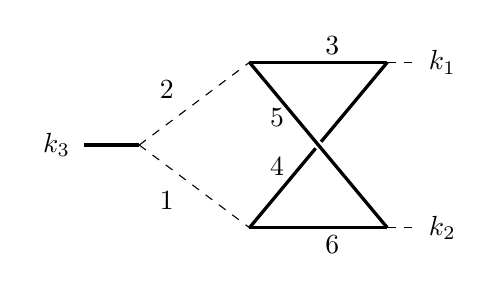
\begin{tikzpicture}[scale=0.7]
		 \draw [black, very thick] (-2,0) to (-3,0);
		\draw [black, dashed] (-2,0) to (-0,1.5);
		\draw [black, dashed] (-2,0) to (-0,-1.5);
		\draw [black,very thick] (0,1.5) to (2.5,-1.5);
		\draw [black,very thick] (0,-1.5) to (1.20,-0.06);
		\draw [black,very thick] (1.30,0.06) to (2.5,1.5);
		\draw [black,very thick] (0,1.5) to (2.5,1.5);
		\draw [black,very thick] (0,-1.5) to (2.5,-1.5);
%		\draw [black, thick] (2.5,-1.5) to (3.0,-1.5);
%		\draw [black, thick] (2.5,1.5) to (3.0,1.5);
                	\draw [black, dashed] (2.5,-1.5) to (3.0,-1.5);
		\draw [black, dashed] (2.5,1.5) to (3.0,1.5);
		\node[text width=0.5cm, text centered ] at (-1.5,-1.) {$1$};
		\node[text width=0.5cm, text centered ] at (-1.5,1.) {$2$};
		\node[text width=0.5cm, text centered ] at (1.5,1.8) {$3$};
		\node[text width=0.5cm, text centered ] at (1.5,-1.8) {$6$};
		\node[text width=0.5cm, text centered ] at (0.5,-0.4) {$4$};
		\node[text width=0.5cm, text centered ] at (0.5,0.5) {$5$};
		\node[text width=0.5cm, text centered ] at (-3.5,0.0) {$k_3$};
		\node[text width=0.5cm, text centered ] at (3.5,-1.5) {$k_2$};
		\node[text width=0.5cm, text centered ] at (3.5,1.5) {$k_1$};
	\end{tikzpicture}
	\caption{The roast chicken graph. Dashed lines are massless
          propagators and solid lines are massive propagators. The
          external momenta $k_i$ satisfy $k_1+k_2+k_3=0$ and $k_1^2=k_2^2=0$.}\label{fig:roastchicken}
\end{figure}

We set $m=1$ and define $2k_1 \cdot k_2 = X$. We have
\begin{equation}
	\mathbf U_{\chickenDiag} = (x_1+x_2)(x_3+x_4+x_5+x_6)+(x_3+x_4)(x_5+x_6),
\end{equation}
\begin{multline}
\mathbf F _{\chickenDiag}(X)=\left((x_3+x_4+x_5+x_6)x_1x_2+x_1x_3x_5+x_2x_4x_6\right) X
\cr
+\left(x_3+x_4+x_5+x_6\right) 	\mathbf U_{\chickenDiag} 
\end{multline}

The integrand of the Feynman integral is the twisted differential form

\begin{equation}
\Omega_{\chickenDiag} ={	\mathbf U_{\chickenDiag}^{6-3\delta} \over \mathbf (F _{\chickenDiag}(X))^{6-2\delta}}\,\left(	\mathbf U_{\chickenDiag}^3\over \mathbf F _{\chickenDiag}(X)^2\right)^\epsilon\,\Omega^{(0)}_6.
\end{equation}

 \begin{equation}
	\label{eq:roastchicken}
	\mathscr{L}^\epsilon_{\chickenDiag}=(16+X)X^2\left(d\over dX\right)^2+(2 (X+8) \epsilon +7 X+80) X{d\over dX} +4 (X+6) \epsilon +4 (2 X+15)
      \end{equation}
%-----------------------------------------------------------------------
\subsection{The four-point planar and non-planar double boxes graph}\label{sec:doubleboxes}
We show how to derive differential equation for  the massless box and massless double-box integrals in 
dimension $D=4-2\epsilon$. Unlike previous cases,  these integrals are divergent in four
dimensions so the $\epsilon=0$ integral are not defined.
%



\subsubsection{The massless planar double-box graph}

\begin{figure}[h]\centering
	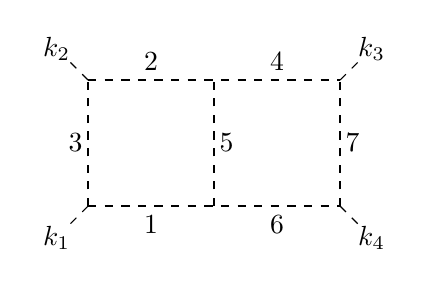
\begin{tikzpicture}[scale=0.8]
		\draw[dashed](-1,-1)--(-1.3,-1.3);
		\draw[dashed](3,-1)--(3.3,-1.3);
		\draw[dashed](3,1)--(3.3,1.3);
		\draw[dashed](-1,1)--(-1.3,1.3);
		\draw[dashed,thick](-1,1)--(3,1);
		\draw[dashed,thick](-1,-1)--(3,-1);
		\draw[dashed,thick](-1,-1)--(-1,1);
		\draw[dashed,thick](1,-1)--(1,1);
		\draw[dashed,thick](3,-1)--(3,1);
		\node[text width=0.5cm, text centered ] at (-1.2,0) {$3$};
		\node[text width=0.5cm, text centered ] at (3.2,0) {$7$};
		\node[text width=0.5cm, text centered ] at (0,-1.3) {$1$};
		\node[text width=0.5cm, text centered ] at (2,-1.3) {$6$};
		\node[text width=0.5cm, text centered ] at (2,1.3) {$4$};
		\node[text width=0.5cm, text centered ] at (1.2, 0) {$5$};
		\node[text width=0.5cm, text centered ] at (0,1.3) {$2$};
		\node[text width=0.5cm, text centered ] at (-1.5,1.5){$k_2$};
		\node[text width=0.5cm, text centered ] at (3.5,1.5){$k_3$};
		\node[text width=0.5cm, text centered ] at (3.5,-1.5){$k_4$};
		\node[text width=0.5cm, text centered ] at (-1.5,-1.5){$k_1$};
	\end{tikzpicture} 
	\caption{The planar massless double-box graphs. The massless
          external momenta $k_i$ satisfy $k_1+\cdots +k_4=0$ and
          $k_i^2=0$. The labels of the graph give the index of the
          edge variable $x_i$. }\label{fig:doublebox}
	 \end{figure}
%
The graph polynomials associated to the massless double-box graph in
fig.~\ref{fig:doublebox} are given by
\begin{align}
	\label{e:DoubleBoxgraphpolynomials}
	\textbf{U}_{\Box\!\Box}&=(x_1+x_2+x_3)(x_4+x_5+x_6)+(x_1+\cdots+x_6)x_7,\\
	\nonumber  \textbf{F}_{\Box\!\Box}(s,t)&=-t x_3x_5x_7-s\left( (x_1+x_2+x_3) x_4x_6+(x_4+x_5+x_6)x_1x_2+(x_1+x_4)(x_2+x_6)x_7\right)
\end{align}
with the twisted differential in $D=4-2\epsilon$ in the projective
space $\mathbb P^6$
\begin{equation}\label{e:OmegaDoubleBox}
	\Omega_{\Box\!\Box}^\epsilon(s,t)=   {\textbf{U}_{\Box\!\Box}  \over
		\textbf{F}_{\Box\!\Box}(s,t)^{3}}\left(\textbf{U}_{\Box\!\Box}^3\over \textbf{F}^2_{\Box\!\Box}(s,t)\right)^\epsilon\,\Omega_0^{(7)}
\end{equation}
we work with the single scale form $\tilde
\Omega_{\Box\!\Box}^\epsilon(X)=(-s)^{3+2\epsilon}
\Omega_{\Box\!\Box}^\epsilon(s,Xs)$
with the result
\begin{equation}\label{e:PF2box}
	\mathscr{L}_{\Box\!\Box}^\epsilon=(1+X)X^2 \left(d\over
	dX\right)^2+(2+3X+\epsilon) X{d\over dX}+X-\epsilon-2\epsilon^2.
\end{equation}



\subsubsection{The massless non-planar double-box graph}

\begin{figure}[h]\centering
 
	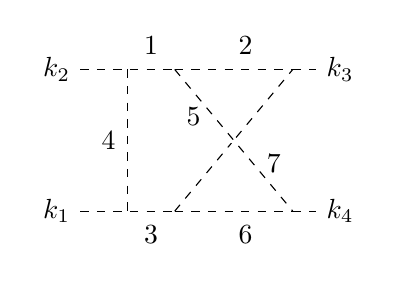
\begin{tikzpicture}[scale=0.6]
          \draw [black, dashed] (-2,1.5) to (0,1.5);
          		\draw [black, dashed] (-2,-1.5) to (0,-1.5);
		\draw [black,dashed] (-1,1.5) to (-1,-1.5);
		\draw [black,dashed] (0,1.5) to (2.5,-1.5);
		\draw [black,dashed] (0,-1.5) to (1.20,-0.06);
		\draw [black,dashed] (1.30,0.06) to (2.5,1.5);
                \draw [black,dashed] (0,1.5) to (2.5,1.5);
		\draw [black,dashed] (0,-1.5) to (2.5,-1.5);
		\draw [black,dashed] (2.5,-1.5) to (3.0,-1.5);
		\draw [black,dashed] (2.5,1.5) to (3.0,1.5);
                \node[text width=0.5cm, text centered ] at (-1.4,0) {$4$};
		\node[text width=0.5cm, text centered ] at (2.1,-0.5) {$7$};
		\node[text width=0.5cm, text centered ] at (-0.5,-2) {$3$};
		\node[text width=0.5cm, text centered ] at (1.5,-2) {$6$};
		\node[text width=0.5cm, text centered ] at (1.5,2) {$2$};
		\node[text width=0.5cm, text centered ] at (0.4, 0.5) {$5$};
		\node[text width=0.5cm, text centered ] at (-0.5,2) {$1$};
		\node[text width=0.5cm, text centered ] at (-2.5,1.5){$k_2$};
		\node[text width=0.5cm, text centered ] at (3.5,1.5){$k_3$};
		\node[text width=0.5cm, text centered ] at (3.5,-1.5){$k_4$};
		\node[text width=0.5cm, text centered ] at (-2.5,-1.5){$k_1$};
	\end{tikzpicture}
	\caption{The non-planar massless double-box graphs. The massless
          external momenta $k_i$ satisfy $k_1+\cdots +k_4=0$ and
          $k_i^2=0$. The labels of the graph give the index of the
          edge variable $x_i$. }\label{fig:npdoublebox}
\end{figure}



\begin{equation}
  \textbf{U}_{\DBoxNP}=(x_1+x_3+x_4)(x_2+x_5+x_6+x_7)+(x_2+x_7)(x_5+x_6) 
 \end{equation}
 and
 \begin{multline}
  \textbf{F}_{\DBoxNP}(s,t)=s\left(x_1x_3(x_2+x_5+x_6+x_7)+x_1x_6x_7+x_2(x_3x_5-x_4x_6)\right)\cr+t x_4 (x_5 x_7-x_2  x_6)
 \end{multline}
we work with the single scale differential form\lNote{myabe some of these examples to appendix?}
 \begin{equation}
  \tilde \Omega^\epsilon_{\DBoxNP}=  (-s)^{3+2\epsilon}  {\textbf{U}_{\DBoxNP}  \over
		\textbf{F}_{\DBoxNP}(s,Xs)^{3}}\left(\textbf{U}_{\DBoxNP}^3\over \textbf{F}^2_{\DBoxNP}(s,sX)\right)^\epsilon\,\Omega_0
 \end{equation}
the differential operator is
 \begin{equation}
   \label{eq:3}
   \mathscr{L}_{\DBoxNP}^\epsilon=(1+X)^2X^2\left(d\over dX\right)^2+(1+X)(1+2X)  (2+\epsilon) X{d\over dX} +2 X(X+1)
   +\left(2 X(X+1)-1\right) \epsilon-2 \epsilon ^2
 \end{equation}

 %-------------------------------------------------------------------------
\subsection{The Witten ice-cream cone diagram}\label{sec:Wittenicecream}
%
%
\begin{figure}\centering
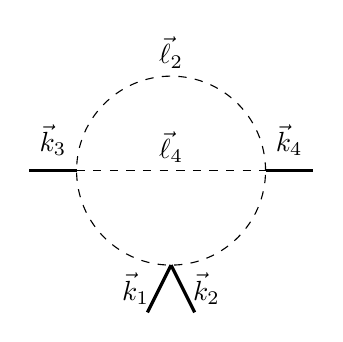
\begin{tikzpicture}[scale=0.6]
\node at (0, 2.5) {$\vec \ell_2$};
\node at (0, 0.5) {$\vec \ell_4$};
\filldraw [color = black, fill=none, dashed] (0,0) circle (2cm);
\draw [ black,dashed] (-2,0) to (2,0);
%\filldraw [black] (2,0) circle (2pt);
%\filldraw [black] (0,-2) circle (2pt);
%\filldraw [black] (-2,0) circle (2pt);
\draw [ black,very thick] (-2,0) to (-3,0);
\draw [ black,very thick]  (3,0) to (2,0);
\draw [ black,very thick] (0,-2) to (0.5,-3);
\draw [ black,very thick] (0,-2) to (-0.5,-3);
\node at (-2.5, 0.65) {$\vec k_3$};
\node at (2.5, 0.65) {$\vec k_4$};
\node at (-0.75, -2.5) {$\vec k_1$};
\node at (0.75, -2.5) {$\vec k_2$};
\end{tikzpicture}
\caption{The Witten ice-cream cone graph in momentum space}
\end{figure}

We turn to the Witten ice-cream cone in analytic regularisation
entering the two-loop correction to the cosmological correlator
between conformally coupled field analysed in Section~5.3.4 of~\cite{Chowdhury:2023arc}.
The cosmological correlator is the integration over the energy of the
two-loop flat space integral analytically regulated
\begin{equation}
  I_{\IceCream}= \int \frac{d^{4}L_{2}d^{4}L_{4}}{(L_2^2)^{1+\kappa}(L_4^2)^{1+\kappa}((L_4+L_2+Q)^2)^{1+\kappa}((L_4+L_2+\tilde Q)^2))^{1+\kappa} }  
\end{equation}
where $\vec k_1+\vec k_2+\vec k_3+\vec k_4=0$ and $Q=(\omega_3,\vec
k_3)$ and $\tilde Q=(\omega_4,-\vec k_4)$.
The parametric representation is given by the integration 
$
  I_{\IceCream} = \int_{\Delta_4} \Omega_{\IceCream}^\kappa
$
over the domain $\Delta_4=\{x_i\geq0,1\leq i\leq 4\}$ of the
differential form
\begin{equation}
  \Omega_{\IceCream}^\kappa= {\pi^4\Gamma(4\kappa)\over
    \Gamma(1+\kappa)^4} \,{1\over \textbf{U}_{\IceCream}^{2} }
  \left(\prod_{i=1}^4 {x_i\textbf{U}_{\IceCream}\over \textbf{F}_{\IceCream}}  \right)^\kappa\,\Omega_4^{(0)}\,,
\end{equation}
with the graph polynomials
\begin{equation}
    \textbf{U}_{\IceCream}=x_1x_2+(x_1+x_2)(x_3+x_4),
  \end{equation}
  and
  \begin{equation}
    \textbf{F}_{\IceCream}=x_1x_2\left(x_3 Q^2+x_4 \tilde
      Q^2\right)+(x_1+x_2)x_3x_4 (Q-\tilde Q)^2.
  \end{equation}
  Setting  $u= Q^2/(Q-\tilde Q)^2$ and $v=\tilde Q^2/(Q-\tilde Q)^2$
  one finds the following Gr\"obner basis of differential operators
  \pvnote{give the mathematica file}
  \begin{align}
  \mathscr{L}_1&=\left(1-u
   -v\right) v\left(\partial\over\partial v\right)^{2} -2u
                 v{\partial\over\partial u}{\partial\over\partial
                 v}-(3 \kappa+1)u {\partial\over\partial u}+(3 \kappa
                 (1-  u-2  v)-v){\partial\over\partial v}-8 \kappa ^2,\cr
  \mathscr{L}_2&=     -u\left(\partial\over\partial u\right)^{2}    +v\left(\partial\over\partial v\right)^{2}       -3 \kappa
   {\partial\over\partial u}+3 \kappa
                 {\partial\over\partial v},\cr
 \mathscr{L}_3&=       2v^2 \left((u-v)^2+1-2(u+v)\right) \left(\partial\over
                \partial v\right)^3\cr
                &+v\left(9 \kappa  \left(u^2-2 u
                (v+1)+(v-1)^2\right)-u^2+u (2-8 v)+9 v^2-8
                v-1\right)\left(\partial\over\partial
                  v\right)^2\cr
                  &+u(\kappa-1)\left(\kappa  (9 u-5 v-9)+3
                    u+v-3\right){\partial\over\partial u}\cr
                    &+\Big(\kappa ^2 \left(9 u^2-u (11 v+18)-2 v^2-25 v+9\right)-3 \kappa  \left(3 u^2+6 u (v-1)-9
                      v^2+2 v+3\right)\cr
                      &+v (-u+5 v+1)\Big){\partial\over\partial v}+24 (\kappa -1) \kappa ^2 (u-v-1)\,.
  \end{align}
%%%%%%%%%%%%%%%%%%%%%%%%%%%%%%%%%%%%%%%%%%%%%%%%%%%%%%%%%%%%%%%
\section{Three- and higher-loop examples}\label{sec:higherloop}

We now turn to the higher-loop cases. We first discuss the all equal
mass case and then a numerical example at three-loop order with all
possible mass configurations.

%----------------------------------------------------------------------
\subsection{Minimal differential operator for higher-loop sunset}
\begin{comment}
\begin{figure}[h]
  \centering
      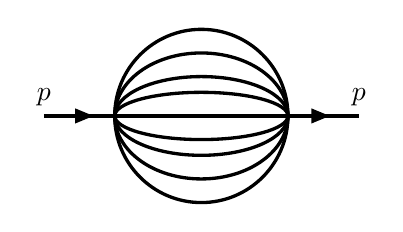
\begin{tikzpicture}[baseline=(x)]
        \begin{feynman}
       \vertex (x);
      \vertex[left=2cm of x,label=$p$](c1l);
      \vertex[right=2cm of x,label=$p$](c1r);
%      \tikzfeynmanset{every vertex=dot}
        \vertex [left=1cm  of x] (xl);
        \vertex [right=1cm  of x] (xr);
        \draw [color = black, fill=none, very thick] (xl)  -- (xr);
        \draw [color = black, fill=none, very thick] (c1l)  -- (xl);
        \draw [color = black, fill=none, very thick] (xr)  -- (c1r);
        \diagram* {
         (c1l) -- [fermion] (xl);
         (xr) -- [fermion] (c1r);
         (xl)  [color = black, fill=none, very thick] -- (xr);
                                };
                              \end{feynman}
                                           \begin{pgfonlayer}{bg}
                                             \draw  [color = black, fill=none, very thick]  (x) circle (1.1cm);
                                              \draw  [color = black, fill=none, very thick] (x) ellipse (1.1cm
                                              and .8cm);
                                                \draw  [color = black, fill=none, very thick] (x) ellipse
                                                (1.1cm and .5cm);
                                                  \draw  [color =
                                                  black, fill=none,
                                                  very thick]  (x) ellipse (1.1cm and .3cm);
                        \end{pgfonlayer}
                   \end{tikzpicture}
  \caption{Multi-loop sunset}
  \label{fig:sunset}
\end{figure}
\end{comment}
\begin{figure}[h]
	\centering
	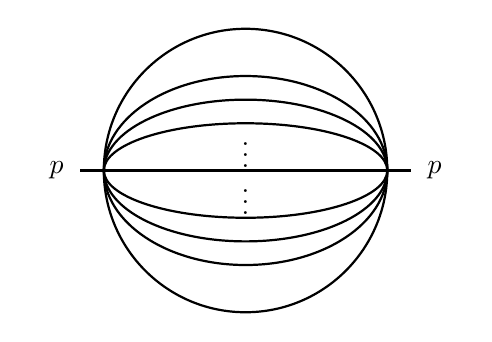
\begin{tikzpicture}[scale=0.6]
		\draw[thick] (0,0) ellipse (3cm and 3cm);
		\draw[thick] (0,0) ellipse (3cm and 2.cm);
		\draw [thick](0,0) ellipse (3cm and 1.5cm);
		\draw [thick](0,0) ellipse (3cm and 1.cm);
		\draw[thick] (-3.5,0)--(3.5,0);
		\node[text width=0.5cm, text centered ] at (0,-.5) {$\vdots$};
		\node[text width=0.5cm, text centered ] at (0,0.5) {$\vdots$};
		\node [text width=0.5cm, text centered ] at (-4,0)
                {$p$};
                	\node [text width=0.5cm, text centered ] at (4,0) {$p$};
%		\node [text width=0.5cm, text centered ] at (0,-2.2){$1$};
%		\node [text width=0.5cm, text centered ] at (0,-1.2){$2$};
%		\node [text width=0.5cm, text centered ] at (0,1.2){$L$};
%		\node [text width=1.5cm, text centered ] at (0,2.2){$L+1$};
	\end{tikzpicture} 
	\caption{Multi-loop sunset}
  \label{fig:sunset}
\end{figure}

A class of examples we will consider is  
the $n-1$-loop sunset integral with $n\geq2$ in $D=2-2\epsilon$ dimensions. Eq.\eqref{e:OmegaTwistDimReg} for this case reads
\begin{equation}
  I^{\epsilon}_{\su(n-1)}(\vec m,t,\epsilon)= \int_{\Delta_n} \Omega^{\epsilon}_{\su(n-1)}(\vec m,t,\epsilon)  ; \quad
  \Omega^\epsilon_{\su(n-1)}(\vec m, t,\epsilon)={\Omega^{(n)}_0\over
    \textbf{F}_{n-1}(t)}\left(\textbf{U}_{n-1}^n\over \textbf{F}_{n-1}(t)^{n-1}\right)^\epsilon
\end{equation}
with
\begin{align}
  \textbf{ U}_{n-1}&= x_1\cdots x_n\sum_{i=1}^n {1\over x_i}\,, \cr
      \textbf{   F}_{n-1}(t)&= \textbf{U}_{n-1} \sum_{i=1}^n m_i^2x_i-t x_1\cdots x_n \, .
\end{align}
Notice that $\textbf{U}_{n-1}^n/ \textbf{F}_{n-1}(t)^{n-1}$ is an homogeneous
rational function  of degree
0 in $(x_1,\dots,x_n)$. As usual the differential form is defined in
the complement of the vanishing locus of the denominator in $\mathbb P^{n-1}\backslash\{\textbf{F}_{n-1}(t)=0\}$.
In $D=2$ dimension ($\epsilon=0$) we have a rational  differential form
$ \Omega_{\su(n-1)}^{\epsilon}(\vec m,t,0)$. The Picard-Fuchs operator has been
given up to six loop  for $\epsilon=0$ and it is in agreement with the Feynman integral
being a (relative) period of a Calabi-Yau  manifold of complex dimension $n-2$~\cite{Bloch:2013tra,Bloch:2014qca,Bloch:2016izu,Bourjaily:2019hmc,Bonisch:2020qmm,Bonisch:2021yfw,Candelas:2021lkc,Forum:2022lpz}.


%----------------------------------------------------------------------   
   \subsubsection{The all equal mass case}\label{sec:highersunset1mass}
Already in $D=2$ dimensions, for the sunset integral from three loop
and higher  the Griffiths-Dwork algorithm had to be adapted because of
the non-isolated singularities of integrand. This was achieved
in~\cite{Lairez:2022zkj} by using syzygies. The resolution of the
linear system in eq.~\eqref{e:sysCFU} takes into account the syzygies
when including the $\epsilon$ dependent factor.   The resolution of
the linear system is optimised with the use of the program {\tt
  FiniteFlow}~\cite{Peraro:2019svx}.


   
For the all equal mass case $m_1=\cdots =m_{l+1}=1$ we find the sunset
Feynman integral satisfies the differential equation
\begin{equation}
  \mathscr{L}_{\su(l)}^\epsilon I_\su(\{1,\dots,1\},t,\epsilon)=
  -(l+1)! {\Gamma(1+\epsilon)^l\over \Gamma(1+l\epsilon)}
\end{equation}
with
\begin{equation}
  \mathscr{L}_{\su(l)}^{\epsilon} =\sum_{r=0}^{l}  \mathscr{L}_{\su(l)}^{r} \epsilon^r
\end{equation}
where the differential operator is $ \mathscr{L}_{\su(l)}^{r}$ is of
order $l-r$. The Picard-Fuchs operator $ \mathscr{L}_{\su(l)}^{0}$ is
the one derived in~\cite{Vanhove:2014wqa} up to five-loops (see as well~\cite{Bonisch:2020qmm,Pogel:2022yat,Pogel:2022ken,Pogel:2022vat}).

The results for the differential equation are given on the {\tt
  SageMath} worksheet \href{Sunset-1mass-Epsilon.ipynb}{Sunset-1mass-Epsilon.ipynb}.
%-------------------------------------------------------------------------


	% sunset integral in general dimensions

\subsubsection{The three-loop generic mass cases}\label{sec:threeloop}

For the three-loop sunset with different masses we find the following
results which are as well given on the  {\tt
  SageMath} worksheet \href{Sunset-Threeloop-Epsilon.ipynb}{Sunset-Threeloop-Epsilon.ipynb}. With the notation of Section~4 of~\cite{Lairez:2022zkj}:
%
\begin{itemize}
\item  {\bf Case~$[4]$:} The all equal mass case $m_1=m_2=m_3=m_4$ has already been
  discussed in the previous section. The $\epsilon^0$ operator was derived and analysed in~\cite{Vanhove:2014wqa,Bloch:2014qca,Pogel:2022yat}. For $ \epsilon \ne 0$, the Picard-Fuchs operator reads
   \end{itemize}
  \begin{multline}
    \mathscr{L}_\su^{[4],\epsilon}=
    -(t - 16)  (t - 4)  t^2\left(d\over dt\right)^3 - 6  (t^3 -
                              15  t^2 + 32  t)  \left(d\over dt\right)^2 - (7  t^2 - 68  t +
                              64)  \left(d\over dt\right) - t + 4\cr
                              +\epsilon \left(-6  (t - 10  ) t^2 \left(d\over dt\right)^2 -
      6  (3  t - 20  ) t \left(d\over dt\right) +18- 6  t 
      \right)\cr
    +\epsilon^2\left(-(11  t^2 -
      28  t - 64)  \left(d\over dt\right) - 11  t + 14\right)+ \epsilon^3\left(-6  t - 12\right)
  \end{multline}

\begin{itemize}

  \item   {\bf Case~$[31]$:} For two different masses $m_1=m_2=m_3 \neq m_4$ the
  Picard-Fuchs operator is of order 5 and has the following $\epsilon$ dependence
  \begin{equation}
    \mathscr{L}^{[31],\epsilon}_\su=       \sum_{r=0}^1 \epsilon^r
    \mathscr{L}^{[31],r}_{5}+  \sum_{r=0}^4 \epsilon^{2+r}   \mathscr{L}^{[31],r}_{4-r} \, ,
  \end{equation}
  where  $ \mathscr{L}^{[31],r}_{n}$ are of order $n$.
  The order $\epsilon^0$ operator factorizes as
  \begin{equation}
         \mathscr{L}^{[31],0}_{5}=   \mathscr{L}^{[31],0}_{a,1} \mathscr{L}^{[31],\epsilon}_\su \, , 
       \end{equation}
        where  $ \mathscr{L}^{[31],0}_{a,1}$ is a  first order operator
       and $\mathscr{L}^{[31],0}_\su$ is the fourth order
       Picard-Fuchs operator of the
       three-loop sunset integral with mass configuration $[31]$ (see 
       in Section~4.3 of~\cite{Lairez:2022zkj}).
       The coefficient of the highest order term $(d/dt)^5$    is given by
       \begin{multline}
                   \mathscr{L}^{[31],\epsilon}_\su\Big\vert_{(d/dt)^5}=
                   t^3  (t-(m_1-m_4)^2)(t-(m_1+m_4)^2)(t-(3m_1+m_4)^2) \cr\times (t-(3m_1-m_4)^2)
            q^{[31]}(t,\epsilon)      .
                 \end{multline}
                 The $\epsilon$ dependence appears only in the
                 apparent singularities determined by the polynomial
                 $q^{[31]}(t,\epsilon)$ of degree 3 in $t$ and 1 in $\epsilon$.
\item   {\bf Case~$[22]$:} For two different masses $m_1=m_2\neq m_3 = m_4$ the
  Picard-Fuchs operator has order 6 and the $\epsilon$ expansion 
  \begin{equation}
    \mathscr{L}_\su^{[22],\epsilon}=     \sum_{r=0}^3 \epsilon^r
    \mathscr{L}^{[22],r}_{6}+  \sum_{r=0}^5 \epsilon^{4+r}   \mathscr{L}^{[22],r}_{5-r} \, ,
  \end{equation}
  where  $ \mathscr{L}^{[22],r}_{n}$ are 
  operators of order $n$.
  The order $\epsilon^0$ operator factorizes as
  \begin{equation}
         \mathscr{L}^{[22],0}_{6}=   \mathscr{L}^{[22],0}_{a,1} \mathscr{L}^{[22],0}_{b,1}\mathscr{L}^{[22],0}_\su \,,
       \end{equation}
       where  $ \mathscr{L}^{[22],0}_{a,1}$ and $
       \mathscr{L}^{[22],0}_{b,1}$ are first order operators. 
        $\mathscr{L}^{[22],0}_\su$ is the fourth order operator for the
       three-loop sunset integral with mass configuration $[22]$ given  Section~4.3 of~\cite{Lairez:2022zkj}.
    The coefficient of the highest order term $(d/dt)^6$    is given by
       \begin{multline}
                   \mathscr{L}^{[22],\epsilon}_\su\Big\vert_{(d/dt)^6}=
                   t^4(t-(2m_1)^2)(t-(2m_4)^2)(t-(2m_1+2m_4)^2)\cr\times(t-(2m_1-2m_4)^2)
                   \, q^{[22]}(t,\epsilon).
                 \end{multline}
                 The $\epsilon$ dependence appears only in the
                 apparent singularities determined by the polynomial
                 $q^{[22]}(t,\epsilon)$ of degree 4 in $t$ and $3$ in $\epsilon$.
     \item   {\bf Case~$[211]$:} For three different masses $m_1=m_2\neq m_3 \neq m_4$ the
  Picard-Fuchs operator has order 7 and has the $\epsilon$ expansion
  \begin{equation}
    \mathscr{L}^{[211],\epsilon}_\su=       \sum_{r=0}^8 \epsilon^r
    \mathscr{L}^{[211],r}_{7}+  \sum_{r=0}^6 \epsilon^{9+r}   \mathscr{L}^{[22],r}_{6-r} \,,
  \end{equation}
   where  $ \mathscr{L}^{[211],r}_{n}$ 
  are operators of order $n$.
    The order $\epsilon^0$ operator factorizes as
  \begin{equation}
         \mathscr{L}^{[211],0}_{7}=   \mathscr{L}^{[211],0}_{a,1}  \mathscr{L}^{[211],0}_{b,1} \mathscr{L}^{[211],0}_{c,1}\mathscr{L}^{[211],0}_\su \,,
       \end{equation}
        where  $ \mathscr{L}^{[211],0}_{a,1}$,  $
        \mathscr{L}^{[211],0}_{b,1}$ and  $ \mathscr{L}^{[211],0}_{c,1}$ are  first order operators
       and $\mathscr{L}^{[211],0}_\su$ is the fifth order Picard-Fuchs operator the
       three-loop sunset integral with mass configuration $[211]$
       given Section~4.3 of~\cite{Lairez:2022zkj}.   The coefficient of the highest order term $(d/dt)^6$    is given by
       \begin{multline}
                   \mathscr{L}^{[211],\epsilon}_\su\Big\vert_{(d/dt)^6}=
                   t^5\left(t-(m_{1}-m_{2})^2\right) \left(t-(m_{1}+m_{2})^2\right)\cr\times
   \left(t-(m_{1}+m_{2}-2 m_{4})^2\right) \left(t-(m_{1}-m_{2}+2
   m_{4})^2\right) \left(t-(-m_{1}+m_{2}+2 m_{4})^2\right)\cr\times
   \left(t-(m_{1}+m_{2}+2 m_{4})^2\right)
                   \, q^{[211]}(t,\epsilon).
                 \end{multline}
                 The $\epsilon$ dependence appears only in the
                 apparent singularities determined by the polynomial
                 $q^{[211]}(t,\epsilon)$ of degree 9 in $t$  and 7 in $\epsilon$.
  \item   {\bf Case~$[1111]$:} For four different masses $m_1\neq m_2\neq m_3 \neq m_4$ the
  Picard-Fuchs operator has order 11 and has the $\epsilon$ expansion 
  \begin{equation}
    \mathscr{L}_\su^{[1111],\epsilon}=     \sum_{r=0}^{16}\epsilon^r
    \mathscr{L}^{[1111],r}_{11}+\sum_{r=0}^{11} \epsilon^{16+r}  \mathscr{L}^{[1111],\epsilon}_{11-r}\, .
  \end{equation}
    The order $\epsilon^0$ operator factorizes as
  \begin{equation}
         \mathscr{L}^{[1111],0}_{0,11}=   \mathscr{L}^{[1111],0}_{a_1,1}  \cdots  \mathscr{L}^{[1111],0}_{a_5,1}   \mathscr{L}^{[1111],0}_{\su}\,,
       \end{equation}
        where  $ \mathscr{L}^{[1111],\epsilon}_{a_1,1},\dots,  \mathscr{L}^{[1111],\epsilon}_{a_5,1}$ are  first order operators
       and $\mathscr{L}^{[1111],0}_{\su}$ is the sixth  order  Picard-Fuchs operator for the
       three-loop sunset integral with mass configuration $[1111]$
       given in~\cite{Lairez:2022zkj}.
        The coefficient of the highest order term $(d/dt)^{11}$    is given by
       \begin{multline}
                   \mathscr{L}^{[1111],\epsilon}_\su\Big\vert_{(d/dt)^{11}}=
                   t^{11}\left(t-(m_{1}+m_{2}-m_{3}-m_{4})^2\right) \cr\times
   \left(t-(m_{1}-m_{2}+m_{3}-m_{4})^2\right)
   \left(t-(m_{1}+m_{2}+m_{3}-m_{4})^2\right) \cr\times
   \left(t-(m_{1}-m_{2}-m_{3}+m_{4})^2\right)
   \left(t-(m_{1}+m_{2}-m_{3}+m_{4})^2\right)\cr\times
   \left(t-(m_{1}-m_{2}+m_{3}+m_{4})^2\right)
   \left(t-(-m_{1}+m_{2}+m_{3}+m_{4})^2\right) \cr\times
   \left(t-(m_{1}+m_{2}+m_{3}+m_{4})^2\right)
                   \, q^{[1111]}(t,\epsilon).
                 \end{multline}
                 The $\epsilon$ dependence appears only in the
                 apparent singularities determined by the polynomial
                 $q^{[1111]}(t,\epsilon)$ of degree 17 in
                 $t$ and 16 in $\epsilon$.
     \end{itemize}
%%%%%%%%%%%%%%%%%%%%%%%%%%%%%%%%%%%%%%%%%%%%%%%%%%%%%%%%%%%%%%%%%%
\section{Discussion}
%
In Section~\ref{sec:griff-dwork-reduct}, we have presented an
algorithm for deriving inhomogeneous differential equations satisfied by Feynman
integrals. At each derivative order the
 procedure consists of solving the linear systems~\eqref{e:sysCFU} in order to
determine the coefficients $c_{a_1,\dots,a_r}(\underline z)$ and the 
inhomogeneous term $\beta_\Gamma$ in~\eqref{e:PFOmegaGeneric}. Our
work introduces an explicit dependence on $\epsilon$ or $\kappa$ so it is worth discussing  its effect on the minimal differential
operator and on the singularities of the differential equations.
%

%------------------------------------------------------------------------
\subsection{Minimal order of the differential operator}
\label{sec:minim-order-diff}

In the examples studied in this work we have found the following:

\begin{itemize}
	\item  For the $n-1$-loop
	sunset integrals, the number of irreducible master integrals 
	is $2^{n}-n-1$~\cite{Kalmykov:2012rr,Bitoun:2017nre}. 
%
%	
	\begin{itemize}  \item The minimal differential Picard-Fuchs operator for the all
		equal mass case has order  $n-1$ .
		\item At one-loop $n=2$ we have an operator of order 1, at two-loop
		$n=3$ an operator of order 4 and at three-loop $n=4$ with generic
		mass configuration the Picard-Fuchs operator
		as   order 11.  We see that when $\epsilon\neq0$  the order of the
		Picard-Fuchs operator saturates bound given by the number of
		irreducible master.
	\end{itemize}
	\item For the two-loop ice-cream cone the number of irreducible
          master four.
          \begin{itemize}
            \item The generic mass and kinematics the minimal order of the $\epsilon$ deformed minimal Picard-Fuchs
	operator is four.
        \item For special kinematic configurations  the ice-cream cone
          Picard-Fuchs operator  is three which is smaller than the
          number of masters.
        \end{itemize}
        \end{itemize}
This leads us to conjecture that 
 for general kinematics the minimal (i.e. not
factorisable) $\epsilon$-deformed Picard-Fuchs operator has 
the same order
as the number of master integrals. But for special kinematics the minimal
order is smaller.
%
The reduction of order arises when the integrand has more
singularities or more symmetries:
\begin{itemize}
  \item {\bf More singularities:} In the case of
massless internal lines or massless external kinematics, extra
singularities arise thus reducing the genus of the
singular locus of the integral. This has for  consequence a lowering
of the order  minimal differential operator. 
\item {\bf More symmetries:}
Another situation is when special choices of kinematic
configurations the integrand of the Feynman integral produce extra
symmetries in the space of projective variables $\underline
x$. This leads to new relations between independent (period) integrals, which reduce the number of independent integrals. A typical case is the
reduction order of the sunset integral according the mass
configurations as given in~\cite{Bloch:2014qca,Lairez:2022zkj,Bonisch:2021yfw,Bonisch:2020qmm,Pogel:2022vat}.
\end{itemize}


This reduction of order can be
understood by the factorisability of the Picard-Fuchs operator
\begin{equation}
  \mathscr{L}_{\rm generic} \stackrel{\rm restriction}{\longrightarrow}
  \hat{\mathscr{L}}_{\rm restricted}   = \mathscr{L}_1 \circ\mathscr{L}_{\rm minimal} \,.
\end{equation}
For instance in Section~4 of~\cite{Lairez:2022zkj} it has been shown
how the multi-loop sunset Picard-Fuchs operator factorizes under
internal mass identifications. Moreover,
%
%As well 
the minimal order differential operator for the all equal
mass $L$-loop sunset is $L$. This is much smaller than 
$2^{L+1}-\binom{L+2}{\left\lfloor \frac{L+2}{2}\right\rfloor }$ for generic
mass configurations~\cite{Lairez:2022zkj} which is the number of
master integrals~\cite{Bitoun:2017nre}.
The reason being that the Feynman integral for the all equal mass
configuration has more symmetries.  

We have noticed that the algorithm presented in this work produces the 
the minimal  differential operator and does not need any factorisation
of the differential operator, to the contrary to the procedure
presented in~\cite{Pogel:2022vat}. 
%
%

Unfortunately, the order drop is not detected by  either the
computation of the Euler characteristic of complement of graph
hypersurface in the projective space of the edge variables, nor the
computation using the critical points of the
Lee-Pomeransky representation~\cite{Lee:2013hzt}   nor the
Baikov
representation~\cite{Frellesvig:2017aai,Frellesvig:2019uqt,Cacciatori:2021nli}.
For instance in ~\cite{Marzucca:2023gto} it was explained how a hidden involution symmetry of the
two-loop non-planar double-box allows to identify the hyperelliptic
curve of genus 2 when the use of the Baikov representation gave a
curve of genus 3.
It is shown in~\cite{Doran:2023yzu}, using
a detailed  algebraic-geometrical analysis, that all planar two-loop
integrals are either period of rational curves, elliptic curve or genus
2 hyperelliptic curves or minimal order two or four respectively.

%------------------------------------------------------------------------
\subsection{The regulator dependence}
\label{sec:epsilon-dependence}

%
For a differential equation
\begin{equation}\label{e:PFconclusion}
c_N(z)  {d^Nf(z)\over dz^N}+\cdots + c_0(z) f(z)=0,
\end{equation}
the roots of $c_N(z)$ are the singularities of the differential
equation. A root of $c_N(z)$ where the solution $f(z)$ is
regular is called an apparent singularity. A root of $c_N(z)$
where the solution has a singularity is a real (See 
Section~16.4 of~\cite{Ince} for details). 
%
For the case of Feynman integrals the non-apparent singularities
of~\eqref{e:PFconclusion} are the roots of the
discriminant of the singular locus of the integrand of  Feynman
integrals~\cite{Doran:2023yzu}.

We have noticed that the dimensional regulator $\epsilon$ appears only in  the
apparent singularities of the differential operator
$\mathscr{L}_z^\epsilon$. This means that the  $\epsilon$ deformation
does not change the position of the real singularities but it affects
the local behaviour (the monodromy) of the solution near the
singularity.
%
The physical interpretation of this is that the kinematic
singularities (the position of the thresholds
and pseudo-thresholds) of a Feynman integral are independent of the
space-time dimension. However,  the local behaviour of the integral near
the thresholds and pseudo-thresholds does change with the space-time
dimension. The latter has been used with great success
when decomposing amplitudes using the generalized unitarity method~\cite{Bern:2011qt}.

%------------------------------------------------------------------------
\section{Conclusion}\label{sec:conclusion}
We have presented a generalisation of the Griffiths-Dwork reduction
for deriving the differential operator acting on Feynman integrals in
dimensional regularisation or analytic regularisation. The algorithm
makes a special use of the fact that the twist from the regularisation
is the power of a degree zero homogeneous rational function in the
edge variables. The procedure amounts to
solving linear systems which is done using {\tt
  FiniteFlow} routines~\cite{Peraro:2019svx}.

We have applied the algorithm to various cases and derived the
inhomogeneous partial differential equations satisfied by the integrand of the Feynman integral in parametric representation.
In dimensional regularisation we have confirmed that the order the
differential operators is smaller or equal to the number of master
integrals. The order of the differential operators is lower for the cases of the kinematic invariants where the integrand
presents more symmetry (equal masses, special kinematics,\dots) or
more singularities (massless internal or external states). Something
that was already noticed in the case of finite integrals~\cite{Lairez:2022zkj}  but stays
true for the regulated integrals.

One motivation for presenting this algorithm is its application to
Feynman integral in analytical regularisation which enters the evaluation of the cosmological
correlators~\cite{Heckelbacher:2022hbq,Chowdhury:2023khl,Chowdhury:2023arc}. 


%%%%%%%%%%%%%%%%%%%%%%%%%%%%%%%%%%%%%%%%%%%%%%%%%%%%%%%%%%%%%%%
\section*{Acknowledgements}
We would like to thank Pierre Lairez,  Eric Pichon-Pharabod  for discussions. We also thank Tiziano Peraro for correspondence on the use of {\tt
	FiniteFlow}. P.V. thanks the LAPTh for hospitality when this
      work has been completed.
The work of P.V. has received funding from the ANR grant ``SMAGP''
ANR-20-CE40-0026-01. P.V. acknowledges support of the Institut Henri
Poincar\'e (UAR 839 CNRS-Sorbonne Universit\'e), and LabEx CARMIN
(ANR-10-LABX-59-01). The work of LDLC is  supported by 
the European Research Council under grant ERC-AdG-885414. 
%\pvnote{Leonardo put your grants}


%%%%%%%%%%%%%%%%%%%%%%%%%%%%%%%%%%%%%%%%%%%%%%%%%%%%%%%%%%%%%%%
\appendix\section{The Bessel representation for the sunset graphs}\label{sec:bessel}


Following the steps in Section~8 of~\cite{Vanhove:2014wqa}
gives the following Bessel integral representation for the multiloop
sunset integral in  $D=2-2\epsilon$ dimensions
\begin{multline}
  I_{\su(n-1)}^\epsilon(\vec m,t,\epsilon)=
  {2^{(n-1) (1-\epsilon)} t^{\epsilon\over2} \over    (m_1\cdots m_{L+1})^{\epsilon}
  \Gamma(1+(n-1)\epsilon)}\cr\times\int_0^\infty I_{-\epsilon}(\sqrt{t} x)
  \prod_{i=1}^{L+1}K_{-\epsilon}(m_ix)\,  x^{1+\epsilon(n-1)}dx.
\end{multline}
This integral representation is valid for   for $t<(m_1+\cdots +m_{n})^2$.
%
For $x\to0$ we have
\begin{equation}
  \lim_{x\to0} I_{-\epsilon}(x)\simeq \left(x\over2\right)^{\epsilon};    \qquad
  \lim_{x\to0} K_{-\epsilon}(x)   \simeq \left(x\over2\right)^{\epsilon}
\end{equation}
and the integral converges as long as $2+(n-1)\epsilon>0$ which is the
condition $D=2-2\epsilon< 2n/(n-1)$ for the absence of ultraviolet divergences
for the $n-1$-loop massive sunset.

Using this representation and applying the creative telescoping
algorithm~\cite{Chyzak,Chyzak2,bostan2013creative,Koutchan} we have checked the results obtained the
extended Griffiths-Dwork reduction.
The creative telescoping algorithm builds an annihilator
\begin{equation}
  \mathscr{T}(t,\partial_t; x,\partial_x)= \mathscr{L}(t,\partial_t)+ \mathscr{C}(  t,\partial_t; x,\partial_x)
\end{equation}
of the integrand
$f(t,x):= I_{-\epsilon}(\sqrt{t} x)
  \prod_{i=1}^{L+1}K_{-\epsilon}(m_ix)\,  x^{1+\epsilon(n-1)}$
such that
\begin{equation}
      \mathscr{T}(t,\partial_t; x,\partial_x) f(t,x)=\mathscr{L}(t,\partial_t)i(t,x)+ \mathscr{C}(  t,\partial_t; x,\partial_x) f(t,x)=0
    \end{equation}
    implying that $\mathscr{L}(t,\partial_t)f(t,x)$ is the operator acting
    on the integral because the domain of integration is independent
    of $t$.
On an ordinary laptop, the results for the all equal mass case and up to twenty loops order, are obtained in
a few second to a few minutes. Which is of the same order of time as
the generalised Griffiths-Dwork reduction presented in the main text
of this work.
    
%%%%%%%%%%%%%%%%%%%%%%%%%%%%%%%%%%%%%%%%%%%%%%%%%%%%%%%%%%%%%%%
\begin{thebibliography}{99}


\bibitem{Golubeva} V. A. Golubeva, ``Some Problems In The Analytic
  Theory Of Feynman Integrals'' , Russ. Math. Surv. {\bf 31} 139 (1976)

\bibitem{Pham} F.~Pham, ``Introduction \`a l'\'etude topologique des
  singularit\'es de Landau'', Paris : Gauthier-Villars; 1967

\bibitem{Panzer:2015ida}
E.~Panzer,
``Feynman Integrals and Hyperlogarithms,''
% doi:10.18452/17157
Thesis: PhD Humboldt U. (2015)
[arXiv:1506.07243 [math-ph]].

  \bibitem{Duhr:2019wtr}
C.~Duhr,
``Function Theory for Multiloop Feynman Integrals,''
Ann. Rev. Nucl. Part. Sci. \textbf{69} (2019), 15-39
%doi:10.1146/annurev-nucl-101918-023551

\bibitem{Mizera:2019ose}
S.~Mizera,
``Status of Intersection Theory and Feynman Integrals,''
PoS \textbf{MA2019} (2019), 016
%doi:10.22323/1.383.0016
[arXiv:2002.10476 [hep-th]].

\bibitem{Travaglini:2022uwo}
G.~Travaglini, A.~Brandhuber, P.~Dorey, T.~McLoughlin, S.~Abreu, Z.~Bern, N.~E.~J.~Bjerrum-Bohr, J.~Bl\"umlein, R.~Britto and J.~J.~M.~Carrasco, \textit{et al.}
``The SAGEX review on scattering amplitudes,''
J. Phys. A \textbf{55} (2022) no.44, 443001
%doi:10.1088/1751-8121/ac8380
[arXiv:2203.13011 [hep-th]].

\bibitem{Doran:2023yzu}
C.~F.~Doran, A.~Harder, E.~Pichon-Pharabod and P.~Vanhove,
``Motivic Geometry of Two-Loop Feynman Integrals,''
[arXiv:2302.14840 [math.AG]].


  \bibitem{Brown:2009ta}
Francis Brown.
\newblock {On the periods of some {F}eynman integrals}.
\newblock 10 2009.
\newblock [arXiv:0910.0114]  

\bibitem{Bloch:2014qca}
Spencer Bloch, Matt Kerr, and Pierre Vanhove.
\newblock {A Feynman integral via higher normal functions}.
\newblock {\em Compos. Math.}, 151(12):2329--2375, 2015.
\newblock [arXiv:1406.2664] 

\bibitem{Bloch:2016izu}
Spencer Bloch, Matt Kerr, and Pierre Vanhove.
\newblock {Local mirror symmetry and the sunset Feynman integral}.
\newblock {\em Adv. Theor. Math. Phys.}, 21:1373--1453, 2017.
\newblock [arXiv:1601.08181]

\bibitem{Bourjaily:2018ycu}
J.~L.~Bourjaily, Y.~H.~He, A.~J.~Mcleod, M.~Von Hippel and M.~Wilhelm,
``Traintracks Through Calabi--Yau Manifolds: Scattering Amplitudes Beyond Elliptic Polylogarithms,''
Phys. Rev. Lett. \textbf{121} (2018) no.7, 071603
%doi:10.1103/PhysRevLett.121.071603
[arXiv:1805.09326 [hep-th]].
  

\bibitem{Bourjaily:2019hmc}
J.~L.~Bourjaily, A.~J.~McLeod, C.~Vergu, M.~Volk, M.~Von Hippel and M.~Wilhelm,
``Embedding Feynman Integral (Calabi-Yau) Geometries in Weighted Projective Space,''
JHEP \textbf{01} (2020), 078
%doi:10.1007/JHEP01(2020)078
[arXiv:1910.01534 [hep-th]].

\bibitem{Bourjaily:2018yfy}
J.~L.~Bourjaily, A.~J.~McLeod, M.~von Hippel and M.~Wilhelm,
``Bounded Collection of Feynman Integral Calabi--Yau Geometries,''
Phys. Rev. Lett. \textbf{122} (2019) no.3, 031601
%doi:10.1103/PhysRevLett.122.031601
[arXiv:1810.07689 [hep-th]].

\bibitem{Klemm:2019dbm}
A.~Klemm, C.~Nega and R.~Safari,
``The $l$-loop Banana Amplitude from Gkz Systems and Relative Calabi-Yau Periods,''
JHEP \textbf{04} (2020), 088
%doi:10.1007/JHEP04(2020)088
[arXiv:1912.06201 [hep-th]].

\bibitem{Bonisch:2020qmm}
K.~B\"onisch, F.~Fischbach, A.~Klemm, C.~Nega and R.~Safari,
``Analytic structure of all loop banana integrals,''
JHEP \textbf{05} (2021), 066
%doi:10.1007/JHEP05(2021)066
[arXiv:2008.10574 [hep-th]].


\bibitem{Bonisch:2021yfw}
K.~B\"onisch, C.~Duhr, F.~Fischbach, A.~Klemm and C.~Nega,
``Feynman Integrals in Dimensional Regularization and Extensions of Calabi-Yau Motives,''
JHEP \textbf{09} (2022), 156
%doi:10.1007/JHEP09(2022)156
[arXiv:2108.05310 [hep-th]].

\bibitem{Bourjaily:2022bwx}
J.~L.~Bourjaily, J.~Broedel, E.~Chaubey, C.~Duhr, H.~Frellesvig, M.~Hidding, R.~Marzucca, A.~J.~McLeod, M.~Spradlin and L.~Tancredi, \textit{et al.}
``Functions Beyond Multiple Polylogarithms for Precision Collider Physics,''
[arXiv:2203.07088 [hep-ph]].


  \bibitem{Forum:2022lpz}
A.~Forum and M.~von Hippel,
``A Symbol and Coaction for Higher-Loop Sunrise Integrals,''
[arXiv:2209.03922 [hep-th]].

\bibitem{Duhr:2022pch}
C.~Duhr, A.~Klemm, F.~Loebbert, C.~Nega and F.~Porkert,
``Yangian-Invariant Fishnet Integrals in 2 Dimensions as Volumes of Calabi--Yau Varieties,''
[arXiv:2209.05291 [hep-th]].

\bibitem{Frellesvig:2023PM}
H. Frellesvig, R. Morales, and M. Wilhelm
``Calabi-Yau meets Gravity: A Calabi-Yau three-fold at fifth post-Minkowskian order,''
[arXiv:2312.11371 [hep-th]].

\bibitem{Pogel:2023zyd}
S.~P\"ogel, X.~Wang and S.~Weinzierl,
``Feynman Integrals, Geometries and Differential Equations,''
[arXiv:2309.07531 [hep-th]].
  

\bibitem{Heckelbacher:2022hbq}
T.~Heckelbacher, I.~Sachs, E.~Skvortsov and P.~Vanhove,
``Analytical Evaluation of Cosmological Correlation Functions,''
JHEP \textbf{08} (2022), 139
%doi:10.1007/JHEP08(2022)139
[arXiv:2204.07217 [hep-th]].

\bibitem{Heckelbacher:2022fbx}
T.~Heckelbacher, I.~Sachs, E.~Skvortsov and P.~Vanhove,
``Analytical Evaluation of AdS$_{4}$ Witten Diagrams as Flat Space Multi-Loop Feynman Integrals,''
JHEP \textbf{08} (2022), 052
%doi:10.1007/JHEP08(2022)052
[arXiv:2201.09626 [hep-th]].

\bibitem{Chowdhury:2023arc}
C.~Chowdhury, A.~Lipstein, J.~Mei, I.~Sachs and P.~Vanhove,
``The Subtle Simplicity of Cosmological Correlators,''
[arXiv:2312.13803 [hep-th]].


\bibitem{Griffiths_1969}
P.~A. Griffiths.
\newblock On the periods of certain rational integrals.
\newblock {Ann. of Math.}, {\bf 90} (1969), 460--541.


  \bibitem{Griffith1} Griffiths, P.A.: The Residue Calculus and Some
    Transcendental Results in Algebraic Geometry, I. Presented at the
    (1966)

    \bibitem{Griffith2} 
    Griffiths, P.A.: ``The Residue Calculus And Some Transcendental
    Results In Algebraic Geometry, II''. Proceedings of the National
    Academy of Sciences. 55, 1392-1395
    (1966). https://doi.org/10.1073/pnas.55.6.1392 

\bibitem{Dwork_1962}
B.~Dwork.
\newblock On the zeta function of a hypersurface.
\newblock {Inst. Hautes \'Etudes Sci. Publ. Math.} {\bf 12} (1962) 5--68.

\bibitem{Dwork_1964}
B.~Dwork.
\newblock On the zeta function of a hypersurface: {{II}}.
\newblock {Ann. of Math.}, {\bf 80} (1964) 227--299.
  
\bibitem{Vanhove:2018mto}
P.~Vanhove,
``Feynman Integrals, Toric Geometry and Mirror Symmetry,''
%doi:10.1007/978-3-030-04480-0\_17
[arXiv:1807.11466 [hep-th]].
  
\bibitem{Lairez:2022zkj}
P.~Lairez and P.~Vanhove,
``Algorithms for Minimal Picard-Fuchs Operators of Feynman Integrals,''
Lett. Math. Phys. \textbf{113} (2023) no.2, 37
%doi:10.1007/s11005-023-01661-3
[arXiv:2209.10962 [hep-th]].



  \bibitem{nakanishi1971graph}
Noboru Nakanishi,
\newblock {\em Graph theory and Feynman integrals}, volume~11.
\newblock Routledge, 1971.

  
  \bibitem{Vanhove:2014wqa}
P.~Vanhove,
``The Physics and the Mixed Hodge Structure of Feynman Integrals,''
Proc. Symp. Pure Math. \textbf{88} (2014), 161-194
%doi:10.1090/pspum/088/01455
[arXiv:1401.6438 [hep-th]].


 \bibitem{Bogner:2010kv}
C.~Bogner and S.~Weinzierl,
``Feynman Graph Polynomials,''
Int. J. Mod. Phys. A \textbf{25} (2010), 2585-2618
%doi:10.1142/S0217751X10049438
[arXiv:1002.3458 [hep-ph]].

\bibitem{Weinzierl:2022eaz}
Stefan Weinzierl.
\newblock Quantum field theory.
\newblock In {\em Feynman Integrals: A Comprehensive Treatment for Students and
  Researchers}, pages 101--133. Springer, 2022.
\newblock [arXiv:2201.03593] 
  
\bibitem{bek}
Spencer Bloch, H{\'e}l{\`e}ne Esnault, and Dirk Kreimer.
\newblock On motives associated to graph polynomials.
\newblock {\em Communications in mathematical physics},
267(1):181--225, 2006.
\newblock [arXiv:math/0510011] 

\bibitem{Speer}  E. R. Speer, ``Generalized Feynman Amplitudes,'' vol. 62 of Annals of Mathematics Studies. Princeton University Press, New Jersey, Apr., 1969.
  


   \bibitem{Aomoto1} K.~Aomoto, ``Les \'equations aux diff\'erences
     lin\'eaires et les int\'egrales des fonctions multiformes'',
     J. Fac. Sci. Univ. Tokyo, 22(3), 271-297  (1975)

  \bibitem{Aomoto} K.~Aomoto, ``On vanishing of cohomology attached to
    certain many valued meromorphic functions'', J. Math. Soc. Japan
    27(2): 248-255 (1975)

  
\bibitem{Aomoto_1982}  K.~Aomoto, ``Configurations and Invariant Gauss-Manin Connections of Integrals I.'' Tokyo Journal of Mathematics 5, 249-287. https://doi.org/10.3836/tjm/1270214894

    \bibitem{AomotoBook} K.~Aomoto, K. and M.~Kita, , ``Theory of Hypergeometric Functions,'' Springer Monographs in Mathematics, Springer-Verlag, Tokyo, 2011
\bibitem{Mizera:2017rqa}
S.~Mizera,
``Scattering Amplitudes from Intersection Theory,''
Phys. Rev. Lett. \textbf{120} (2018) no.14, 141602
%doi:10.1103/PhysRevLett.120.141602
[arXiv:1711.00469 [hep-th]].

\bibitem{Frellesvig:2019uqt}
H.~Frellesvig, F.~Gasparotto, M.~K.~Mandal, P.~Mastrolia, L.~Mattiazzi and S.~Mizera,
``Vector Space of Feynman Integrals and Multivariate Intersection Numbers,''
Phys. Rev. Lett. \textbf{123} (2019) no.20, 201602
%doi:10.1103/PhysRevLett.123.201602
[arXiv:1907.02000 [hep-th]].
    
\bibitem{Cacciatori:2021nli}
S.~L.~Cacciatori, M.~Conti and S.~Trevisan,
``Co-Homology of Differential Forms and Feynman Diagrams,''
Universe \textbf{7} (2021) no.9, 328
doi:10.3390/universe7090328
[arXiv:2107.14721 [hep-th]].

\bibitem{Munch:2023ifm}
H.~J.~Munch,
``Evaluating Feynman Integrals Using D-modules and Tropical Geometry,''
[arXiv:2401.00891 [hep-th]].
  
\bibitem{Brunello:2023rpq}
G.~Brunello, V.~Chestnov, G.~Crisanti, H.~Frellesvig, M.~K.~Mandal and P.~Mastrolia,
``Intersection Numbers, Polynomial Division and Relative Cohomology,''
[arXiv:2401.01897 [hep-th]].

\bibitem{Teschke:2024bct}
T.~Teschke,
``General Relativity from Intersection Theory and Loop Integrals,''
[arXiv:2401.01920 [hep-th]].
  


\bibitem{Kashiwara:1977nf}
M.~Kashiwara and T.~Kawai, \emph{{Holonomic Systems of Linear Differential
		Equations and Feynman Integrals}},
\href{https://doi.org/10.2977/prims/1195196602}{\emph{Publ. Res. Inst. Math.
		Sci. Kyoto} {\bfseries 12} (1977) 131}.

  
  \bibitem{Bitoun:2017nre}
T.~Bitoun, C.~Bogner, R.~P.~Klausen and E.~Panzer,
``Feynman Integral Relations from Parametric Annihilators,''
Lett. Math. Phys. \textbf{109} (2019) no.3, 497-564
%doi:10.1007/s11005-018-1114-8
[arXiv:1712.09215 [hep-th]].

\bibitem{Smirnov:2010hn}
A.~V.~Smirnov and A.~V.~Petukhov,
``The Number of Master Integrals is Finite,''
Lett. Math. Phys. \textbf{97} (2011), 37-44
%doi:10.1007/s11005-010-0450-0
[arXiv:1004.4199 [hep-th]].



\bibitem{Lee:2013hzt}
R.~N.~Lee and A.~A.~Pomeransky,
``Critical Points and Number of Master Integrals,''
JHEP \textbf{11} (2013), 165
%doi:10.1007/JHEP11(2013)165
[arXiv:1308.6676 [hep-ph]].



\bibitem{muller2014picard}
Stefan M{\"u}ller-Stach, Stefan Weinzierl, and Raphael Zayadeh.
\newblock Picard--{F}uchs equations for {F}eynman integrals.
\newblock {\em Communications in Mathematical Physics},
326(1):237--249, 2014.
\newblock [arXiv:1212.4389]
  
\bibitem{delaCruz:2019skx}
L.~de la Cruz,
``Feynman Integrals as A-Hypergeometric Functions,''
JHEP \textbf{12} (2019), 123
%doi:10.1007/JHEP12(2019)123
[arXiv:1907.00507 [math-ph]].

\bibitem{Klausen:2019hrg}
R.~P.~Klausen,
``Hypergeometric Series Representations of Feynman Integrals by Gkz Hypergeometric Systems,''
JHEP \textbf{04} (2020), 121
%doi:10.1007/JHEP04(2020)121
[arXiv:1910.08651 [hep-th]].
  
\bibitem{Feng:2019bdx}
T.~F.~Feng, C.~H.~Chang, J.~B.~Chen and H.~B.~Zhang,
``Gkz-Hypergeometric Systems for Feynman Integrals,''
Nucl. Phys. B \textbf{953} (2020), 114952
%doi:10.1016/j.nuclphysb.2020.114952
[arXiv:1912.01726 [hep-th]].

\bibitem{Ananthanarayan:2022ntm}
B.~Ananthanarayan, S.~Banik, S.~Bera and S.~Datta,
``Feyngkz: a Mathematica Package for Solving Feynman Integrals Using Gkz Hypergeometric Systems,''
Comput. Phys. Commun. \textbf{287} (2023), 108699
%doi:10.1016/j.cpc.2023.108699
[arXiv:2211.01285 [hep-th]].

\bibitem{Agostini:2022cgv}
D.~Agostini, C.~Fevola, A.~L.~Sattelberger and S.~Telen,
``Vector Spaces of Generalized Euler Integrals,''
[arXiv:2208.08967 [math.AG]].
\bibitem{Munch:2022ouq}
H.~J.~Munch,
``Feynman Integral Relations from Gkz Hypergeometric Systems,''
PoS \textbf{LL2022} (2022), 042
%doi:10.22323/1.416.0042
[arXiv:2207.09780 [hep-th]].
\bibitem{Chestnov:2023kww}
V.~Chestnov, S.~J.~Matsubara-Heo, H.~J.~Munch and N.~Takayama,
``Restrictions of Pfaffian Systems for Feynman Integrals,''
JHEP \textbf{11} (2023), 202
%doi:10.1007/JHEP11(2023)202
[arXiv:2305.01585 [hep-th]].

\bibitem{Mastrolia:2018uzb}
P.~Mastrolia and S.~Mizera,
``Feynman Integrals and Intersection Theory,''
JHEP \textbf{02} (2019), 139
%doi:10.1007/JHEP02(2019)139
[arXiv:1810.03818 [hep-th]].

\bibitem{Muller-Stach:2011qkg}
S.~M\"uller-Stach, S.~Weinzierl and R.~Zayadeh,
``A Second-Order Differential Equation for the Two-Loop Sunrise Graph with Arbitrary Masses,''
Commun. Num. Theor. Phys. \textbf{6} (2012), 203-222
%doi:10.4310/CNTP.2012.v6.n1.a5
[arXiv:1112.4360 [hep-ph]].

  
\bibitem{PutSinger} van der Put, M., and Singer, M. F. Galois Theory of Linear Differential Equations, Vol. 328. Springer: 2003. An electronic version of this book is available at http://www4.ncsu.edu/\~singer/ms\_papers.html.

 \bibitem{vanHoeij} van Hoeij, M. "Factorization of Differential Operators with Rational Functions Coefficients." J. Symb. Comput. Vol. 24. (1997): 537-561.

\bibitem{chyzak2022symbolic}
Fr\'{e}d\'{e}ric Chyzak, Alexandre Goyer, and Marc Mezzarobba.
\newblock Symbolic-numeric factorization of differential operators.
\newblock In {\em Proceedings of the 2022 International Symposium on Symbolic
  and Algebraic Computation}, ISSAC '22, page 73-82, New York, NY, USA, 2022.
Association for Computing Machinery.
\newblock [arXiv:2205.08991]

\bibitem{goyer2021sage}
Alexandre Goyer.
\newblock A {S}age package for the symbolic-numeric factorization of linear
  differential operators.
\newblock {\em ACM Communications in Computer Algebra}, 55(2):44--48,
2021.

\bibitem{Bloch:2013tra}
S.~Bloch and P.~Vanhove,
``The elliptic dilogarithm for the sunset graph,''
J. Number Theor. \textbf{148} (2015), 328-364
%doi:10.1016/j.jnt.2014.09.032
[arXiv:1309.5865 [hep-th]].
  
\bibitem{Peraro:2019svx}
T.~Peraro,
``Finiteflow: Multivariate Functional Reconstruction Using Finite Fields and Dataflow Graphs,''
JHEP \textbf{07} (2019), 031
%doi:10.1007/JHEP07(2019)031
[arXiv:1905.08019 [hep-ph]].


\bibitem{Koutchan} C. Koutschan. ``HolonomicFunctions (user's guide).'' Technical Report 10-01, RISC Report Series, Johannes Kepler University, Linz, Austria, 2010. http://www.risc
.jku.at/research/ combinat/software/HolonomicFunctions/.

  
\bibitem{Caffo:1998du}
M.~Caffo, H.~Czyz, S.~Laporta and E.~Remiddi,
``The Master Differential Equations for the Two Loop Sunrise Selfmass Amplitudes,''
Nuovo Cim. A \textbf{111} (1998), 365-389
[arXiv:hep-th/9805118 [hep-th]].
  
\bibitem{Remiddi:2013joa}
E.~Remiddi and L.~Tancredi,
``Schouten Identities for Feynman Graph Amplitudes; the Master Integrals for the Two-Loop Massive Sunrise Graph,''
Nucl. Phys. B \textbf{880} (2014), 343-377
%doi:10.1016/j.nuclphysb.2014.01.009
[arXiv:1311.3342 [hep-ph]].
  
\bibitem{Adams:2013nia}
L.~Adams, C.~Bogner and S.~Weinzierl,
``The Two-Loop Sunrise Graph with Arbitrary Masses,''
J. Math. Phys. \textbf{54} (2013), 052303
%doi:10.1063/1.4804996
[arXiv:1302.7004 [hep-ph]].

\bibitem{Pogel:2022vat}
S.~P\"ogel, X.~Wang and S.~Weinzierl,
``Bananas of Equal Mass: Any Loop, Any Order in the Dimensional Regularisation Parameter,''
JHEP \textbf{04} (2023), 117
%doi:10.1007/JHEP04(2023)117
[arXiv:2212.08908 [hep-th]].

 

\bibitem{Remiddi:2016gno}
E.~Remiddi and L.~Tancredi,
``Differential equations and dispersion relations for Feynman amplitudes. The two-loop massive sunrise and the kite integral,''
Nucl. Phys. B \textbf{907} (2016), 400-444
%doi:10.1016/j.nuclphysb.2016.04.013
[arXiv:1602.01481 [hep-ph]].


\bibitem{Broadhurst:1987ei}
D.~J.~Broadhurst,
``The Master Two Loop Diagram With Masses,''
Z. Phys. C \textbf{47} (1990), 115-124
  
\bibitem{Adams:2016xah}
L.~Adams, C.~Bogner, A.~Schweitzer and S.~Weinzierl,
``The Kite Integral to All Orders in Terms of Elliptic Polylogarithms,''
J. Math. Phys. \textbf{57} (2016) no.12, 122302
%doi:10.1063/1.4969060
[arXiv:1607.01571 [hep-ph]].

\bibitem{Candelas:2021lkc}
P.~Candelas, X.~de la Ossa, P.~Kuusela and J.~McGovern,
``Mirror Symmetry for Five-Parameter Hulek-Verrill Manifolds,''
[arXiv:2111.02440 [hep-th]].

\bibitem{Pogel:2022yat}
S.~P\"ogel, X.~Wang and S.~Weinzierl,
``The Three-Loop Equal-Mass Banana Integral in \ensuremath{\varepsilon}-factorised Form with Meromorphic Modular Forms,''
JHEP \textbf{09} (2022), 062
%doi:10.1007/JHEP09(2022)062
[arXiv:2207.12893 [hep-th]].


\bibitem{Pogel:2022ken}
S.~P\"ogel, X.~Wang and S.~Weinzierl,
``Taming Calabi-Yau Feynman Integrals: the Four-Loop Equal-Mass Banana Integral,''
Phys. Rev. Lett. \textbf{130} (2023) no.10, 101601
%doi:10.1103/PhysRevLett.130.101601
[arXiv:2211.04292 [hep-th]].


\bibitem{Kalmykov:2012rr}
M.~Y.~Kalmykov and B.~A.~Kniehl,
``Mellin-Barnes Representations of Feynman Diagrams, Linear Systems of Differential Equations, and Polynomial Solutions,''
Phys. Lett. B \textbf{714} (2012), 103-109
%doi:10.1016/j.physletb.2012.06.045
[arXiv:1205.1697 [hep-th]].
  
  \bibitem{Frellesvig:2017aai}
  H.~Frellesvig and C.~G.~Papadopoulos,
  ``Cuts of Feynman Integrals in Baikov Representation,''
  JHEP {\bf 1704} (2017) 083
%  doi:10.1007/JHEP04(2017)083
  [arXiv:1701.07356 [hep-ph]].
  
  \bibitem{Marzucca:2023gto}
R.~Marzucca, A.~J.~McLeod, B.~Page, S.~P\"ogel and S.~Weinzierl,
``Genus Drop in Hyperelliptic Feynman Integrals,''
[arXiv:2307.11497 [hep-th]].

\bibitem{Ince} E.~L.~Ince, ``Ordinary differential equations.''
  Courier Corporation  (1956).
 

  
\bibitem{Bern:2011qt}
Z.~Bern and Y.~t.~Huang,
``Basics of Generalized Unitarity,''
J. Phys. A \textbf{44} (2011), 454003
doi:10.1088/1751-8113/44/45/454003
[arXiv:1103.1869 [hep-th]].



\bibitem{Chowdhury:2023khl}
C.~Chowdhury and K.~Singh,
``Analytic Results for Loop-Level Momentum Space Witten Diagrams,''
[arXiv:2305.18529 [hep-th]].

\bibitem{Chyzak}  Fr\'ed\'eric Chyzak, `` extension of
    Zeilberger's fast algorithm to general holonomic functions'',
Discrete Mathematics, {\bf 217} (1-3) 115-134, 2000.

\bibitem{Chyzak2} Fr\'ed\'eric Chyzak, ``Creative Telescoping for
  Parametrised Integration and Summation'',  Les cours du CIRM,  Vol. 2, no 1 (2011), Course no II, p. 1-37.

\bibitem{bostan2013creative} A. Bostan, P. Lairez, and B. Salvy,
  ''Creative telescoping for rational functions using the
  Griffiths--Dwork method.'' In Proceedings of the 38th international
  symposium on symbolic and algebraic computation (pp. 93-100). 

	
	


\end{thebibliography}



\end{document}
%%% Local Variables:
%%% mode: latex
%%% TeX-master: t
%%% End:
